%===============================================================================
% LaTeX sjabloon voor de bachelorproef toegepaste informatica aan HOGENT
% Meer info op https://github.com/HoGentTIN/bachproef-latex-sjabloon
%===============================================================================

\documentclass{bachproef-tin}

\usepackage{hogent-thesis-titlepage} % Titelpagina conform aan HOGENT huisstijl

%%---------- Documenteigenschappen ---------------------------------------------
% TODO: Vul dit aan met je eigen info:

% De titel van het rapport/bachelorproef
\title{Het gebruik van single board computers als leermiddel voor
    programmeren in het secundair onderwijs.}

% Je eigen naam
\author{Warre Van de Veire}

% De naam van je promotor (lector van de opleiding)
\promotor{Ludwig Stroobant}

% De naam van je co-promotor. Als je promotor ook je opdrachtgever is en je
% dus ook inhoudelijk begeleidt (en enkel dan!), mag je dit leeg laten.
\copromotor{Annick Van Daele}

% Indien je bachelorproef in opdracht van/in samenwerking met een bedrijf of
% externe organisatie geschreven is, geef je hier de naam. Zoniet laat je dit
% zoals het is.
\instelling{---}

% Academiejaar
\academiejaar{2020-2021}

% Examenperiode
%  - 1e semester = 1e examenperiode => 1
%  - 2e semester = 2e examenperiode => 2
%  - tweede zit  = 3e examenperiode => 3
\examenperiode{2}

\usepackage{graphicx}
\graphicspath{{./img/}}

%===============================================================================
% Inhoud document
%===============================================================================

\begin{document}

%---------- Taalselectie -------------------------------------------------------
% Als je je bachelorproef in het Engels schrijft, haal dan onderstaande regel
% uit commentaar. Let op: de tekst op de voorkaft blijft in het Nederlands, en
% dat is ook de bedoeling!

%\selectlanguage{english}

%---------- Titelblad ----------------------------------------------------------
\inserttitlepage

%---------- Samenvatting, voorwoord --------------------------------------------
\usechapterimagefalse
%%=============================================================================
%% Voorwoord
%%=============================================================================

\chapter*{\IfLanguageName{dutch}{Woord vooraf}{Preface}}
\label{ch:voorwoord}

%% TODO:
%% Het voorwoord is het enige deel van de bachelorproef waar je vanuit je
%% eigen standpunt (``ik-vorm'') mag schrijven. Je kan hier bv. motiveren
%% waarom jij het onderwerp wil bespreken.
%% Vergeet ook niet te bedanken wie je geholpen/gesteund/... heeft

Over de jaren heen heb ik een interesse ontwikkelt voor single board computers. Het idee van een volwaardige computer de grote van een creditkaart was iets wat ik vroeger moeilijk kon vatten. Ik zag voorbeelden van smart mirrors en retro spelcomputerkasten, allemaal dankzij single board computers. Jaren later kwam ik opnieuw in contact met single board computers dankzij het YouTube kanaal: Michael Reeves. Deze youtuber maakt gebruik van Raspberry Pi's en Arduino's om absurde robots te maken. In zijn video's verteld hij hoe makkelijk je robots kan maken met behulp van deze single board computers.  Zo maakte hij, tijdens het schrijven van dit onderzoek, een modificatie voor een robot hond van Boston Dynamics. Met deze modificatie kon de robot plots bier plassen. 

Geniaal en geweldig, maar het deed me denken: is programmeren op zo'n single board computer nu echt zo simpel? En zo ja: zouden kinderen dit kunnen gebruiken om te leren programmeren. Allebei mijn ouders zijn leerkracht, dus de connectie maken met onderwijs was makkelijk. Ik heb als kind vaak zelf moeten leren programmeren via YouTube. Een creatief medium zoals een single board computer leek mij ongelofelijk interessant, maar tot mijn verbazing werd dit nog niet zo vaak gebruikt in het huidige onderwijs. Daarom leek mij dit een leuke uitdaging om te bekijken hoe we single board computers kunnen introduceren bij leerkrachten.

Voor mijn onderzoek start, wil ik graag wat mensen bedanken die mij gesteund hebben tijdens het uitwerken:

Ik wil eerst en vooral mijn co-promotor, Annick van Daele bedanken. Haar interesse in mijn bachelorproef en haar zachtaardig karakter heeft mij altijd de motivatie gegeven om op volle toeren verder te werken. Zonder haar steun doorheen het project ging dit onderzoek niet half zo goed zijn geweest. De wereld van het onderwijs is relatief nieuw voor mij. Dus om een gids te hebben doorheen alle vaktermen en details, was ongelofelijk handig. Mevrouw van Daele heeft mij geholpen tot op het einde van mijn onderzoek; met het opzoeken van bronnen, uitleggen van vakjargon, het verbeteren van mijn taalfouten en doorwijzen naar leerkrachten voor mijn proof of concept. Ik ben zeker niet de makkelijkste om mee te werken, maar ze bleef enthousiast en hoopvol. Vanuit de grond van mijn hard, bedankt.

Hierna wil ik mijn promotor, Ludwig Stroobant, bedanken. Dankzij zijn duidelijke feedback en luisterend oor doorheen het project kan ik met veel trots dit document afwerken. In het begin wist ik niet goed waar te starten en wat precies te doen. Gelukkig stond meneer Stroobant altijd klaar om mijn vragen te beantwoorden op een kalme, duidelijke manier. Soms kon ik door de stress het bos door de bomen niet meer zien, maar dankzij meneer Stroobant lukte dit keer op keer opnieuw. Hartelijk bedankt!

Vervolgens moet ik een paar mensen bedanken die mij hebben geholpen doorheen mijn project. Zo wil ik Francis Wyffels bedanken voor zijn inbreng bij de keuze van single board computers. Dankzij zijn input kon ik de Micro:bit mooi klasseren in mijn onderzoek. Ook moet ik Bert van Vreckem bedanken. Dankzij corona had ik nog geen ervaring met LaTeX opgedaan in het tweede jaar. Ik ben hierdoor vaak vastgelopen met mijn bibliografie. Dankzij zijn hulp heb ik dit document mooi kunnen afwerken. Tenslotte wil ik nog de leerkachten bedanken die mij hebben geholpen bij mijn lesvoorbereiding, zeker Saen Callens en Lieve Van Bastelaere. Hun input maakt mijn onderzoek robuust. Ik wil hun bedanken voor hun tijd en interesse.

Tenslotte wil ik mijn vrienden en familie bedanken voor hun steun. Een bachelorproef maken is zeker geen flauwe kul. Gelukkig had ik altijd de support van mijn naasten om verder te werken. Vooral hebben mijn ouders mij vaak geholpen met vanalles en nog wat. Ze stonden altijd klaar voor mij. Ik zal dit nooit vergeten. Hartelijk bedankt!

  
%%=============================================================================
%% Samenvatting
%%=============================================================================

% TODO: De "abstract" of samenvatting is een kernachtige (~ 1 blz. voor een
% thesis) synthese van het document.
%
% Deze aspecten moeten zeker aan bod komen:
% - Context: waarom is dit werk belangrijk?
% - Nood: waarom moest dit onderzocht worden?
% - Taak: wat heb je precies gedaan?
% - Object: wat staat in dit document geschreven?
% - Resultaat: wat was het resultaat?
% - Conclusie: wat is/zijn de belangrijkste conclusie(s)?
% - Perspectief: blijven er nog vragen open die in de toekomst nog kunnen
%    onderzocht worden? Wat is een mogelijk vervolg voor jouw onderzoek?
%
% LET OP! Een samenvatting is GEEN voorwoord!

%%---------- Nederlandse samenvatting -----------------------------------------
%
% TODO: Als je je bachelorproef in het Engels schrijft, moet je eerst een
% Nederlandse samenvatting invoegen. Haal daarvoor onderstaande code uit
% commentaar.
% Wie zijn bachelorproef in het Nederlands schrijft, kan dit negeren, de inhoud
% wordt niet in het document ingevoegd.

\IfLanguageName{english}{%
\selectlanguage{dutch}
\chapter*{Samenvatting}
\lipsum[1-4]
\selectlanguage{english}
}{}

%%---------- Samenvatting -----------------------------------------------------
% De samenvatting in de hoofdtaal van het document

\chapter*{\IfLanguageName{dutch}{Samenvatting}{Abstract}}

In dit onderzoek wordt bekeken als single board computers kunnen gebruikt worden om leerlingen van de eerste graad secundair onderwijs te leren programmeren. In de moderne wereld zijn ICT-skills nog nooit zo noodzakelijk geweest voor elk kind. Veel kinderen worden geboren met een computer in hun schoot. We staan er niet meer bij stil hoe zo'n computer nu werkt. Tijd om daar verandering in te brengen. De Vlaamse overheid kiest er vaak voor om gewoon elk kind een laptop te geven, maar kan het niet anders? Zo'n investering is kostelijk, maar hoeft het zo te zijn?

Deze bachelorproef bekijkt als we single board computers kunnen gebruiken om leerlingen te leren programmeren. Zo onderzoekt het als we een project kunnen uitvoeren die alle eindtermen van de eerste graad secundair onderwijs aftikt, met behulp van een single board computer. De einddoelen voor digitale competentie en wijsheid worden bekeken en opgesomt. Hierna worden, dankzij SWOT-analyses, verschillende single board computers vergeleken en geëvalueerd. Hierna wordt slechts één uitgekozen. Verder zoeken we naar de ideale programmeertaal om te leren programmeren op een single board computer. Ook hierbij gebruiken we SWOT-analyses. Tot slot werken we een lesvoorbereiding uit voor een project die gebruik maakt van de gekozen single board computer en programmeertaal.

Uit het onderzoek vinden we dat de Raspberry Pi de beste kandidaat is voor een single board computer en Python de ideale programmeertaal. Hierna wordt een raadspel uitgewerkt met behulp van een lesvoorbereiding. Hierop wordt er feedback gegeven door leerkrachten van de eerste graad secundair.

We concluderen dat een single board computer kan gebruikt worden in het onderwijs, maar dat het niet de ideale oplossing is. Ook merken we dat Python toch niet de beste programmeertaal blijkt te zijn voor beginnende studenten. Het is dus belangrijk om duidelijk de juiste hardware en software te kiezen wanneer je gaat werken met single board computers. Tenslotte is de doelgroep nog te jong: een uitwerking in Python klinkt realistischer in de tweede graad.

Na het onderzoek vragen we ons af hoe single board computers kunnen evolueren om beter te werken in het onderwijs. Als uitbreiding van dit onderzoek zou er in de toekomst een les kunnen uitgewerkt worden door middel van Scratch in plaats van Python of een uitwerking in de tweede graad.


%---------- Inhoudstafel -------------------------------------------------------
\pagestyle{empty} % Geen hoofding
\tableofcontents  % Voeg de inhoudstafel toe
\cleardoublepage  % Zorg dat volgende hoofstuk op een oneven pagina begint
\pagestyle{fancy} % Zet hoofding opnieuw aan

%---------- Lijst figuren, afkortingen, ... ------------------------------------

% Indien gewenst kan je hier een lijst van figuren/tabellen opgeven. Geef in
% dat geval je figuren/tabellen altijd een korte beschrijving:
%
%  \caption[korte beschrijving]{uitgebreide beschrijving}
%
% De korte beschrijving wordt gebruikt voor deze lijst, de uitgebreide staat bij
% de figuur of tabel zelf.

\listoffigures

% Als je een lijst van afkortingen of termen wil toevoegen, dan hoort die
% hier thuis. Gebruik bijvoorbeeld de ``glossaries'' package.
% https://www.overleaf.com/learn/latex/Glossaries

%---------- Kern ---------------------------------------------------------------

% De eerste hoofdstukken van een bachelorproef zijn meestal een inleiding op
% het onderwerp, literatuurstudie en verantwoording methodologie.
% Aarzel niet om een meer beschrijvende titel aan deze hoofstukken te geven of
% om bijvoorbeeld de inleiding en/of stand van zaken over meerdere hoofdstukken
% te verspreiden!

%%=============================================================================
%% Inleiding
%%=============================================================================

\chapter{\IfLanguageName{dutch}{Inleiding}{Introduction}}
\label{ch:inleiding}

De inleiding moet de lezer net genoeg informatie verschaffen om het onderwerp te begrijpen en in te zien waarom de onderzoeksvraag de moeite waard is om te onderzoeken. In de inleiding ga je literatuurverwijzingen beperken, zodat de tekst vlot leesbaar blijft. Je kan de inleiding verder onderverdelen in secties als dit de tekst verduidelijkt. Zaken die aan bod kunnen komen in de inleiding:

\begin{itemize}
  \item context, achtergrond
  \item afbakenen van het onderwerp
  \item verantwoording van het onderwerp, methodologie
  \item probleemstelling
  \item onderzoeksdoelstelling
  \item onderzoeksvraag
  \item \ldots
\end{itemize}

\section{\IfLanguageName{dutch}{Probleemstelling}{Problem Statement}}
\label{sec:probleemstelling}

Uit je probleemstelling moet duidelijk zijn dat je onderzoek een meerwaarde heeft voor een concrete doelgroep. De doelgroep moet goed gedefinieerd en afgelijnd zijn. Doelgroepen als ``bedrijven,'' ``KMO's,'' systeembeheerders, enz.~zijn nog te vaag. Als je een lijstje kan maken van de personen/organisaties die een meerwaarde zullen vinden in deze bachelorproef (dit is eigenlijk je steekproefkader), dan is dat een indicatie dat de doelgroep goed gedefinieerd is. Dit kan een enkel bedrijf zijn of zelfs één persoon (je co-promotor/opdrachtgever).

\section{\IfLanguageName{dutch}{Onderzoeksvraag}{Research question}}
\label{sec:onderzoeksvraag}

Wees zo concreet mogelijk bij het formuleren van je onderzoeksvraag. Een onderzoeksvraag is trouwens iets waar nog niemand op dit moment een antwoord heeft (voor zover je kan nagaan). Het opzoeken van bestaande informatie (bv. ``welke tools bestaan er voor deze toepassing?'') is dus geen onderzoeksvraag. Je kan de onderzoeksvraag verder specifiëren in deelvragen. Bv.~als je onderzoek gaat over performantiemetingen, dan 

\section{\IfLanguageName{dutch}{Onderzoeksdoelstelling}{Research objective}}
\label{sec:onderzoeksdoelstelling}

Wat is het beoogde resultaat van je bachelorproef? Wat zijn de criteria voor succes? Beschrijf die zo concreet mogelijk. Gaat het bv. om een proof-of-concept, een prototype, een verslag met aanbevelingen, een vergelijkende studie, enz.

\section{\IfLanguageName{dutch}{Opzet van deze bachelorproef}{Structure of this bachelor thesis}}
\label{sec:opzet-bachelorproef}

% Het is gebruikelijk aan het einde van de inleiding een overzicht te
% geven van de opbouw van de rest van de tekst. Deze sectie bevat al een aanzet
% die je kan aanvullen/aanpassen in functie van je eigen tekst.

De rest van deze bachelorproef is als volgt opgebouwd:

In Hoofdstuk~\ref{ch:stand-van-zaken} wordt een overzicht gegeven van de stand van zaken binnen het onderzoeksdomein, op basis van een literatuurstudie.

In Hoofdstuk~\ref{ch:methodologie} wordt de methodologie toegelicht en worden de gebruikte onderzoekstechnieken besproken om een antwoord te kunnen formuleren op de onderzoeksvragen.

% TODO: Vul hier aan voor je eigen hoofstukken, één of twee zinnen per hoofdstuk

In Hoofdstuk~\ref{ch:conclusie}, tenslotte, wordt de conclusie gegeven en een antwoord geformuleerd op de onderzoeksvragen. Daarbij wordt ook een aanzet gegeven voor toekomstig onderzoek binnen dit domein.

\chapter{\IfLanguageName{dutch}{Stand van zaken}{State of the art}}
\label{ch:stand-van-zaken}

% Tip: Begin elk hoofdstuk met een paragraaf inleiding die beschrijft hoe\cite{Hughes,Hughes,Hughes,Hughes}
% dit hoofdstuk past binnen het geheel van de bachelorproef. Geef in het
% bijzonder aan wat de link is met het vorige en volgende hoofdstuk.

% Pas na deze inleidende paragraaf komt de eerste sectiehoofding.


De “State of the art” of de stand van zaken geeft een beeld over de eindtermen en -competenties van programmeren in de eerste graad van het secundair onderwijs, hoe dit in de praktijk al wordt aangepakt, welke single board computer het meest geschikt lijkt voor onze proof of concept en welke programmeertaal we zullen hanteren.

\section{Programmeren in de eerste graad secundair onderwijs}	

\subsection{Onderwijsdecreet}



Het vlaamse onderwijssysteem krijgt zijn vorm door het huidige onderwijsdecreet. Dit decreet houdt de regels en doelen bij die onderwijsinstellingen moet handhaven. Een decreet staat vast en kan enkel vervangen worden met een volledig nieuw decreet. 
Zo is er een wijziging geweest van het onderwijsdecreet in 2018 en die in 2019 van start ging.  


Bij dit nieuwe onderwijsdecreet gaat het om:

\begin{itemize}
    \item Aanvulling en verbetering van een aantal bestaande decreten;
    \item Een reeks maatregelen tot vereenvoudiging: vermindering van administratie en verbetering van juridische teksten;
    \item Een reeks kleinere maatregelen in uitvoering van het Regeerakkoord.
\end{itemize} (\cite{VLOR2020})

Een onderwijsdecreet is meestal getypeerd door zijn eindtermen. Dit zijn minimumdoelen die een leerling moet bereiken om te kunnen afstuderen. Het huidige onderwijsdecreet vertaalt deze eindtermen in sleutelcompetenties. Het voordeel bij het gebruik van competenties is dat deze niet vastgebonden zijn aan een specifiek vak. Hierdoor kunnen meerdere vakken meerdere competenties tackelen en is er meer samenhang in het lessenpakket.(\cite{Vlaanderen2018})

De manier waarop scholen dit toepassen, hangt af van zijn onderwijsverstrekker\footnote{Een koepel in het onderwijs}. De eindtermen worden namelijk geformuleerd per finaliteit:
\begin{itemize}
    \item Doorstroom finaliteit\footnote{Leerlingen voorbereiden om door te stromen naar het hoger onderwijs.}
    \item Dubbele finaliteit\footnote{leerlingen voorbereiden om verder te studeren in het hoger onderwijs of te starten met werken}
    \item Arbeidsmarktfinaliteit\footnote{leerlingen voorbereiden voor te gaan werken of een graduaatsopleiding}
\end{itemize}
Een leerplan is een overzicht van de leerinhoud die in een klas moet worden behandeld. Deze omvat minstens de te bereiken eindtermen. Wanneer nodig, kan de onderwijsverstrekker daaraan doelen toevoegen of accenten leggen. Een leerplan geeft dus in essentie een overzicht van de leerinhouden en doelen. Daarnaast voegt het ook nog didatische werken toe. Deze laatste helpen de leerkrachten de leerdoelen om te zetten naar praktische uitwerkingen Alle scholen in Vlaanderen en Brussel die erkend zijn door het Ministerie van Onderwijs en Vorming zijn verplicht een door de overheid goedgekeurd leerplan te volgen.  Een leerplan kan goedgekeurd worden wanneer de eindtermen en ontwikkelingsdoelen duidelijk en herkenbaar te vinden zijn in het plan.(\cite{Parlement})

Zo heeft men in het katholiek onderwijs gekozen om de opgegeven competenties te vertalen naar een eigen leerplan. De einddoelen staan niet letterlijk verwerkt in dit plan, maar zijn geformuleerd naar eigen leerdoelen. Het gemeenschapsonderwijs neemt letterlijk de competenties over van het huidige onderwijsdecreet en vult deze in hun leerplannen. De competenties worden letterlijk overgenomen. Het is dus duidelijk dat de verschillen in leerplannen potentieel een moeilijkheid kan vormen bij het uitvoeren van dit onderzoek. Deze factor moet dus meegenomen worden.(\cite{Llinkid2019,Smartschool})

\subsection{Digitale competenties en mediawijsheid} 
In het huidige onderwijsdecreet worden eindtermen geformuleerd in exact 16 sleutelcompetenties. Bij het uitdenken van deze competenties is er nadruk gelegd op de verschillende uitdagingen van de 21ste eeuw. Zo ligt er meer nadruk op bepaalde competenties zoals economie, STEM (Sience, Technology, Engineering, Mathematics) en duurzaamheid.(\cite{Vlaanderen2018b})

Voor dit onderzoek is slechts één sleutelcompetentie van belang: Digitale competentie en mediawijsheid. Deze is onderverdeeld in drie duidelijke bouwstenen:
\begin{itemize}
    \item Digitale media en toepassingen gebruiken om te creëren, te participeren en te interageren
    \item Computationeel denken en handelen.
    \item Verantwoord, kritisch en ethisch omgaan met digitale en niet digitale media en informatie.
\end{itemize}
(\cite{Vlaanderen2018a})

Met deze bouwstenen moet een leerling van de eerste graad in staat zijn om met digitale media te werken, kritisch te denken over die digitale media en probleemoplossend te denken. 
Zoals eerder vermeld, gebruikt het katholiek onderwijs zijn eigen leerdoelen, met de opgestelde competenties als basis. Voor de eerste graad secundair onderwijs hebben ze het leerplan ICT - I AB. Dit leerplan wordt onderverdeeld in 3 onderdelen:
\begin{itemize}
    \item Digitale basisvaardigheden
    \item Inzicht in computersystemen
    \item Computationeel denken
\end{itemize}(\cite{Llinkid2019})

Zoals de naam impliceert, zijn deze leerdoelen nauw verbonden aan informatica, maar in de praktijk kunnen de doelen in verschillende vakken aan bod komen. Deze leerdoelen zijn duidelijk niet integraal overgenomen uit de opgegeven digitale competenties, met uitzondering van computationeel denken.
In het gemeenschapsonderwijs worden de sleutelcompetenties wel letterlijk opgenomen. Deze leerdoelen worden in de praktijk voor de eerste graad vooral ingevuld bij de STEM-vakkencluster. (\cite{Smartschool})

Tenslotte wordt er een verschil gemaakt in de manier waarop deze competenties worden geïmplementeerd. Men spreekt bij Digitale competenties en mediawijsheid over transversale leerdoelen. Transversale leerdoelen moeten, naast de inhoudelijke leerdoelen, in samenhang met meerdere vakken gerealiseerd worden. Dit betekent dat alle transversale leerdoelen moeten voorkomen in meerdere vakken of vakken clusters. Dit houdt niet in dat alle transversale leerdoelen in elk vak moet voorkomen, maar deze te vinden zijn in meerdere vakken. Inhoudelijke leerdoelen kunnen daadwerkelijk wel binnen één vak gerealiseerd worden. In het uitwerken van dit onderzoek is er gekozen om het begrip transversaal te laten vallen, waardoor nu ook deze doelen kunnen gerealiseerd worden in één vak \footnote{\url{https://www.klasse.be/114462/basisprincipes-nieuwe-eindtermen/}}.
Hoewel al deze eindtermen zeker belangrijk zijn om de uitdagingen van de 21ste eeuw te kunnen tackelen, zullen ons we in dit onderzoek vooral spitsen op het computationeel denken. Dit is de basis van programmeren en exact hetgeen we willen realiseren in de eerste graad.

\subsection{Computationeel denken} 
Computational thinking (CT) is een term bedacht door Jeannette Wing, die het gebruikt om een geheel van denkvaardigheden, gewoonten en benaderingen te kunnen beschrijven. Die zijn integraal voor het oplossen van complexe problemen met behulp van een computer en breed toepasbaar in de informatiemaatschappij.
Deze term houdt vooral in dat we met computationeel denken, grotere problemen kunnen opsplitsen in kleinere, abstracte probleem. Als we hierna alle kleine problemen succesvol kunnen oplossen, is het grotere probleem ook opgelost. Hierbij maken we gebruiken van algoritmisch en wiskundig denken.

Computationeel denken kan onderverdeeld worden in vier principes:

\begin{itemize}
    \item Decompositie
    \item Patroonherkenning
    \item Abstractie
    \item Algoritmen
\end{itemize} (\cite{Smartschool,Vlaanderen,Llinkid2019})
Decompositie betekent: het opdelen van een probleem in kleinere deelproblemen om zo de complexiteit te verkleinen. Dit soort denken wordt al vaak geïmplementeerd, zoals in het maken van een stappenplan. Als je het zo bekijkt, is “decompositie” een cruciaal deel van programmeren. Zo worden grotere componenten, zoals het maken van een zoekbalk op een website, verdeeld in kleinere sub processen die samenwerken om een geheel functie te geven. In dit geval zou bijvoorbeeld het aanmaken van navigatielinks een onderdeel kunnen zijn. Ook testen schrijven is hier een onderdeel van.
(\cite{Smartschool})

Vervolgens vormt “patroonherkenning” het tweede onderdeel van computationeel denken. Dit kan men oefenen door bijvoorbeeld het soorten en classificeren van gegevens. Opnieuw is dit een cruciale factor in het correct leren programmeren. Als je patronen herkent in bepaalde processen, kan je code schrijven die hergebruikt kan worden in andere plaatsen van de applicatie. Een voorbeeld hiervan is het maken van een confirmatiescherm wanneer je iets zou verwijderen of een belangrijke stap zou uitvoeren in een applicatie.
(\cite{Smartschool})\\

Abstractie is iets moeilijker te vatten, maar heeft hetzelfde doel als decompositie: complexiteit weghalen van een groter project. Dit doet men bij abstractie door de belangrijkste elementen over te nemen en de details even te negeren om tot de kern van een probleem te komen. Zo is het oplossen van een vraagstuk wiskunde of fysica een voorbeeld van abstractie: niet elk detail van een vraagstuk is belangrijk om een oplossing te vinden. Ook bij programmeren is bij het ontwerpen van een oplossing niet elk klein detail van belang. Zo leer je efficiënt omgaan met code en maak je het ook beter leesbaar.
(\cite{Smartschool})

Tenslotte tackelt computationeel denken “algoritmisch denken”. Algoritmen worden vaak gekoppeld aan programmeren en voor een goede reden. Algoritmen zijn namelijk een serie geordende instructies die na elkaar worden uitgevoerd om het probleem op te lossen of om een kleiner doel te bereiken. Een algoritme is dus hetgeen wat al deze stappen bij elkaar houdt. Wanneer je dus alle stappen via decompositie opdeelt, patronen herkent en toepast, onnodige details weghaalt en alle stappen op volgorde uitvoert, heb je een compleet product. Het grote probleem is dus simpelweg omgevormd naar een algoritme met kleinere sub processen. 
(\cite{Smartschool})


Bij de proof of concept van dit onderzoek is het dus noodzakelijk dat alle bovengenoemde aspecten van computationeel denken aanwezig is. Het is uiterst belangrijk om de resultaten van de proof of concept terug te koppelen aan de eindtermen die vernoemd staan in het onderwijsdecreet. Zo kan men evalueren of het gebruik van single board computers daadwerkelijk een plaats heeft in het leren programmeren.


\section{Vergelijking van single board computers}

\subsection{Single Board Computers}

Single board computers zijn kleine mini computers waarvan alle componenten gemonteerd zijn op één enkele printplaat. Deze mini computers zijn zowel compact, goedkoop als flexibel. Zo kan het gebruikt worden voor verschillende doeleinden, van IoT (Internet of Things) apparaten tot simpele garagedeur bedieningen. Maar belangrijker voor dit onderzoek: de single board computer is gemaakt om gebruikt te worden in de klas. Zo willen de uitvinders van de Raspberry Pi bijvoorbeeld de jeugd leren hoe bepaalde technologie werkt en hoe het gebruikt kan worden.
(\cite{ET2012})

Volgens de ontwikkelaars van de Raspberry Pi wordt er minder en minder kritisch nagedacht over hoe technologie werkt. Nu iedereen rondloopt met kant en klare technologie, zoals een smartphone, is er volgens Raspberry minder interesse om te weten hoe zoiets nu werkt. Men vreest hierdoor dat dit verdere innovatie zou kunnen tegenhouden. Daarom is het cruciaal om kinderen en jongeren meer te leren over deze “naakte computers”.(\cite{ET2012})

Volgens Gareth Mitchel \footnote{radiopresentator en lector wetenschappelijke communicatie aan Londen College} is dit idee niet zomaar zonder kritiek. Volgens critici is dit niets meer dan een simpele elektronische kit die men in het verleden ook al gebruikte. Dit zou eerder een stap teruggaan in de tijd dan een innovatieve uitvinding, maar volgens Mitchel is een stap terugzetten een cruciaal deel van het leerproces. Het is juist door het versimpelen van technologie dat we een beter beeld kunnen scheppen over het potentieel ervan. Hierdoor kunnen we de weg vrijmaken voor grotere doorbraken in de toekomst.(\cite{ET2012})

Voor dit onderzoek willen we op zoek gaan naar de meest geschikte single board computer om kinderen grafisch te leren programmeren. Er bestaan ongelooflijk veel verschillende soorten single board computers, elk met hun eigen functies en eigenschappen. Zo bestaan er zelfs krachtige single board computers voor gaming applicaties. Om de lengte van dit onderzoek te beperken zullen we enkel de vergelijking maken tussen de Arduino, Micro Bit en de Raspberry Pi. Deze worden namelijk het meest gebruikt in een educatieve context.

\subsection{Raspberry Pi }

Tijdens de periode van dit onderzoek is de meest bekende single board computer de Raspberry Pi \footnote{\url{https://www.electromaker.io/blog/article/best-single-board-computers}}. Opgericht in 2008  als liefdadigheidsinstelling in het Verenigd Koninkrijk, staat de Raspberry Pi Foundation in voor het verspreiden van computationele en digitale kennis over de hele wereld.
Zo organiseert Raspberry verschillende workshops en events om het potentieel van de Raspberry Pi te demonstreren. Ook moedigt Raspberry verschillende scholen over de hele wereld aan om gebruik te maken van hun technologie in de klas. Zo wil het niet alleen programmeren populair maken, maar wil het ook technologie introduceren in andere wetenschappelijk vakken zoals fysica of chemie.
(\cite{Foundation})


Zoals eerder vermeld in dit onderzoek, vreest de Raspberry Pi Foundation dat de kennis van computers stilaan zou verdwijnen, nu we de computer zelf niet moeten programmeren. Het wil jongeren opnieuw warm maken om bij te leren over de ins en outs van een computer.

Net zoals andere single board computers heeft de Raspberry Pi een goedkope aankoopprijs. Zo koop je een Raspberry Pi 4 Model B met 2GB RAM voor slechts 39,95 euro \footnote{\url{https://www.kiwi-electronics.nl/raspberry-pi-4-model-b-2gb?src=raspberrypi}}. Wanneer je grotere applicaties vlot tegelijk wilt laten draaien, zijn er opties met 4GB en zelfs 8GB RAM. Deze opties zijn echter iets duurder. Zo heeft de 8GB variant een prijskaartje van 87,50 euro\footnote{\url{https://www.raspberrystore.nl/PrestaShop/raspberry-pi-v4/279-raspberry-pi-4b-8gb-765756931199.html?utm_source=RaspberryPi&utm_medium=Shop&utm_campaign=Pi&utm_term=be&src=raspberrypi}}. Nog steeds goedkoop voor een computer, maar misschien toch te duur om massaal in een school aan te kopen. Gelukkig bestaan er goedkopere opties, zoals de Raspberry Pi 3 Model B voor slechts 36,95 euro\footnote{https://yadom.fr/raspberry-pi-3-modele-bp-1gb.html?src=raspberrypi} of de Raspberry Pi voor slechts 10,71 euro\footnote{\url{https://www.sossolutions.nl/raspberry-pi-pico-headers?gclid=Cj0KCQjwwLKFBhDPARIsAPzPi-KTn0mt_aXSp5tb5bKMp8wtOK-3TdIhOoC1gmpO0E6TI8y1Rm6lK-YaAsQSEALw_wcB}}. De laatstgenoemde optie heeft duidelijk minder processing power in vergelijking met de rest, met slechts 512MB aan RAM.
De Raspberry heeft ook twee tot vier USB poorten (afhankelijk van het model), een ethernet kabel voor bedraad internet, ingebouwde draadloze connectiviteit zowel voor wifi als bluetooth en twee micro HDMI-poorten, zodat je makkelijk kan verbinden met 2 schermen tegelijk.

Een single board computer heeft een laag energiegebruik en de Raspberry Pi is geen uitzondering. Het heeft enkel een USB-C of microUSB kabel nodig voor stroom (afhankelijk van het model). Deze zijn makkelijk te verkrijgen, aangezien de meeste smartphones dezelfde oplaadkabels gebruiken. Ook is de Raspberry Pi klein van formaat (85.6mm op 56.5mm). Dankzij dit formaat en het feit dat het weinig energie verbruikt, is er geen nood aan een ventilator om alle componenten koel te houden. Dus is de Pi uiterst stil, zelfs tijdens de grootste processen.(\cite{Foundationa}) 

Tenslotte straalt de Pi uit op vlak van programmeertalen. Zo heeft de Pi zijn eigen besturingssysteem (zoals windows of IoS), genaamd Raspbian OS. Dit zorgt voor een makkelijke instap bij het gebruiken van de Pi. Ook komt het standaard met Python en Scratch: allebei makkelijk te gebruiken programmeertalen. Het hoeft echter daar niet te eindigen, aangezien het ook C++, C en Ruby geïnstalleerd heeft staan. Wanneer dit nog onvoldoende is, kunt u verschillende andere programmeertalen online installeren. Zo ondersteunt de Raspberry Pi zelfs Android applicaties. De Raspberry Pi Foundation heeft zelfs eigen cursussen en kits om de gebruiker te helpen bij elke stap van het programmeer proces \footnote{\url{https://www.raspberrypi.org/learn/}}.(\cite{Pattichis2017,Teja2021,Koelling2016})

Dankzij al deze eigenschappen is de Raspberry Pi een enorm flexibele optie om te gebruiken in de klas. De Pi is wel niet perfect. Zo heeft het bepaalde moeilijkheden die eventueel een obstakel kunnen vormen bij het gebruik ervan in de les. 
De Pi is relatief goedkoop tegenover een klassieke laptop of desktop, maar is wat aan de duurdere kant in vergelijking met andere single board computers. Ook zijn er een beperkt aantal verkopers van de Raspberry Pi en kan je deze enkel online vinden. Je kan ze dus niet makkelijk vinden in een gewone electronicawinkel. 
De Raspberry Pi is ook geen kant en klare technologie: je hebt andere componenten zoals een toetsenbord, een SD-kaart voor interne opslag en een scherm nodig vooraleer je kunt starten met programmeren. Dit kan het prijskaartje flink doen stijgen.

Tenslotte moet je voor het optimale gebruik van de Pi vaak speciale packages downloaden en installeren, waardoor de instap bij het gebruik van de Pi groter is dan andere single board computers. Hierdoor is er dus wat voorbereidingswerk nodig bij het gebruik van een Pi.(\cite{Teja2021})

De Raspberry Pi is dus niet de perfecte single board computer. Het heeft een goede prijsklasse en geniet dankzij zijn naambekendheid en open source software van een grote community van Pi enthousiasten. Hierdoor bestaan er al veel projecten die gebruik maken van de kleine computer. Toch, de nood aan externe toestellen zoals een scherm en een toetsenbord is niet alleen onpraktisch, maar ook prijzig. Het heeft ook concurrentie die stilaan aan bekendheid wint en vaak goedkopere alternatieven biedt, zoals de Arduino. Ook is de Raspberry Pi en andere single board computers nog niet bekend in het onderwijs en zijn leerkrachten over heel de wereld nog sceptisch over deze kleine computers. Er is dus nog ruimte voor een alternatieve single board computer.(\cite{Susan2014})

\subsection{Arduino}

Arduino, opgericht in 2005 in Ivrea (Italië), is bekend voor het maken van de Arduino lijn van microcontrollers. Een microcontroller is een apparaat met een geïntegreerde schakeling (IC) die wordt gebruikt om andere delen van een elektronisch systeem te besturen. Een Arduino kan dus gebruikt worden om een bepaalde input om te vormen naar een nieuwe output. De oprichters van Arduino zochten een oplossing om snel en makkelijk verschillende elektronische componenten, zoals sensoren en motoren, aan elkaar te koppelen via hardware en software. Dit moest ook goedkoop blijven om niemand te limiteren in hun creativiteit. Met die gedachtegang werd de Arduino een waanzinnig succes zowel bij artiesten\footnote{een voorbeeld van een kunstwerk, gemaakt met een Raspberry Pi: \url{https://www.raspberrypi.org/blog/interactive-origami-art-with-raspberry-pi/}} als in het onderwijs. (\cite{Hughes})

De Arduino staat bekend voor zijn makkelijke instap. Met de plug-and-play eigenschap van de Arduino, kan men makkelijk sensoren verbinden met de arduino om zo een input te kunnen registreren. Dankzij de Arduino Integrated Development Environment (IDE) kan men makkelijk deze input omvormen naar een output die kan gestuurd worden naar een output apparaat zoals een motor of zelfs een andere Arduino. Voor de duidelijkheid: een Integrated Development Environment is software die een gebruiker de mogelijkheid geeft om leesbare code te schrijven. Je kan met een Arduino zowel programmeren met de Arduino programmeertaal\footnote{Een variant van C++} als met C of C++. Je kan zelfs andere programmeertalen downloaden.(\cite{Teja2021})

Nog een punt vóór Arduino is zijn beginners vriendelijkheid. Niet alleen omdat de instap kleiner is, maar omdat de Arduino meer bestand is tegen eventuele incidenten. Zoals zijn plug-and-play eigenschap insinueert, kan je makkelijk de stroomkabel verwijderen zonder enige problemen of corruptie aan de bestanden. Alle lopende processen worden namelijk eerst afgesloten voor het apparaat compleet stroom verliest. De Raspberry Pi heeft niet zo’n functie en is dus gevoeliger voor corrupte bestanden bij stroomverlies. Daarnaast zijn zowel de Pi als de Arduino energiezuinig, maar ook hier blinkt de Arduino meer uit.(\cite{Teja2021})

Arduino heeft verschillende prijsklassen. Zijn bekendste model, de Arduino uno, heeft slechts een aankoopprijs van 20 euro. Ook heeft het verschillende starter kits speciaal ontworpen voor educationele toepassingen. Hierdoor staat de Arduino momenteel op de eerste plaats voor de meest geschikte microcontroller van dit onderzoek.

Dus de uitkomst is duidelijk: de Arduino wint het van de Raspberry Pi. Met zijn goedkopere aankoopprijs, kant en klare educationele kits en stroomverlies veiligheid lijkt dit de beste single board computer voor in de les toch? Spijtig genoeg voor de Arduino is dit niet het geval.\\ 

Zoals eerder vermeld is de Arduino eigenlijk geen single board computer, maar een microcontroller. Een belangrijk aspect van de Arduino is het transformeren van input naar output door het gebruik van sensoren, maar deze 'hardware' kan enkel één applicatie tegelijk draaien. Het beschikt ook niet over een besturingssysteem. Tenslotte mist de Arduino bepaalde eigenschappen die nodig zijn om het een single board computer te noemen, zoals USB-poorten, hdmi-ingangen, ethernet slots en eventuele wifi receivers.\\

Vaak worden de Pi en de Arduino vergeleken omdat ze op het eerste zicht dezelfde taken uitvoeren. Het verschil ligt in het feit dat de Pi veel complexere en meerdere applicaties kan draaien juist omdat niet alles geïntegreerd is op één chip. Omdat de Arduino enkel een microcontroller bevat waarvan zowel de RAM als de opslag als de processor geïntegreerd staan op één chip, verliest het de optie om verschillende programma’s tegelijk te draaien.(\cite{Teja2021,Keim2019,FreeCodeCamp2017})

De Arduino valt in dit onderzoek dus uit, aangezien het geen single board computer is. Dit betekent wel nog niet dat de Raspberry Pi de beste optie is voor dit onderzoek. Daarvoor hebben we nog één ander voorbeeld van een single board computer die toch een goede concurrent kan vormen voor de Pi. 


\subsection{Micro:bit }
De Micro:bit, gesponserd door de BBC in Groot-Brittannië, is een leuk stukje tech volledig ontworpen om kinderen en jongeren te leren programmeren. Het is een printplaat met verschillende ingebouwde sensoren. De Micro bit ondersteunt zowel Python als Scratch en Microsoft MakeCode. Dankzij deze verschillende codeertalen kan deze input omgevormd worden naar een concrete actie op de Micro Bit zelf. Zo zijn er bijvoorbeeld een aantal led-lichtjes op de printplaat gemonteerd, om directe feedback te tonen aan de gebruiker. (\cite{Stager2018})

De Micro:bit heeft zoals de vorige, opgesomde voorbeelden een lage energieconsumptie. Wat de Micro:bit zo uniek maakt, zijn de verschillende power opties om de kleine techboard aan de praat te krijgen. Je kan op de klassieke manier een USB-port gebruiken voor stroom, maar ook een battery pack of via de 3V connectoren langs de rand van het toestel. Dit zorgt voor veel flexibiliteit en mobiliteit, iets wat niet kan gezegd worden van de PI.
Dit vernuftig stukje tech beschikt niet enkel over een usb-c connector en wat led-lichtjes. Het heeft een touch-sensor, speaker, radio antenne, 2 analoge knoppen en een microfoon. Hierdoor bespaar je toch wat geld bij het aankopen van sensoren. (\cite{Stager2018})

Net zoals de Pi en de Arduino, heeft de Micro:bit een lage aankoopprijs. Zo koop je een Micro:bit GO v2 voor slechts 37,50 euro\footnote{\url{https://www.bol.com/nl/p/microbit-go-v2/9300000019150594/?bltgh=m-pQlfTCD-xYiTss1eNGrA.2_34.36.ProductTitle}}. Dit geeft de Micro:bit een edge boven de Raspberry Pi, die moeilijker online verkrijgbaar is. De Micro:bit heeft ook een intern geheugen, dus is er geen nood aan het kopen van een SD-kaart als geheugen. Hierdoor heeft de Micro:bit een soortgelijke plug-and-play eigenschap van die de Arduino ook bezit.

Tenslotte, juist omdat het doel van de Micro bit exclusief gericht is op educatie, heeft de Micro:bit een grote bibliotheek aan lessen en projecten. Deze zijn makkelijk te vinden o.a. op de  website van Micro:bit zelf\footnote{\url{https://microbit.org/}}. Hierdoor is het makkelijk voor een leerkracht om zo’n project te implementeren in zijn of haar lessen. Opnieuw een plus punt voor de Micro Bit.

In Groot-Brittannië is er zelfs onderzoek gedaan naar het gebruik van de Microbit om te leren programmeren. Zo hebben alle kinderen van het eerste jaar secundair onderwijs gratis een Micro:bit ontvangen die ze konden gebruiken in de les. Na het onderzoek bleek dat 90 procent van de jongeren een eigen project kon coderen en 88 procent leerde dat coderen niet zo moeilijk bleek te zijn. Zelfs meisjes, die door de stereotypen moeilijker te overhalen zijn om te leren programmeren, werd er een stijging in interesse vastgesteld met niet meer dan 70 procent. Ook leerkrachten ondervonden dat de Micro:bit een plezante en creatieve manier is om kinderen te leren programmeren. (\cite{IW2017})

Spijtig genoeg stoppen hier ook de voordelen van de Micro:bit. Het het grote nadeel waardoor het niet kan winnen van de Raspberry Pi: om te kunnen programmeren met een Micro:bit, heb je een externe computer nodig. Dit zorgt ervoor dat het argument van het prijskaartje volledig wegvalt. Ook kan men argumenteren dat om grafisch te leren programmeren, men geen nood heeft aan een Micro: bit, aangezien al het codeerwerk gebeurt op de externe computer.\cite{Singapore}

Tenslotte is men niet zeker of de Micro Bit kan geclassificeerd worden als een single board computer. Sommige bronnen tonen aan van wel, aangezien het meer componenten bevat dan een Arduino, een typisch voorbeeld van een microcontroller. Andere bronnen beweren dat, door het feit dat het niet kwalificeert als een volledig geïntegreerde computer, het niet kan gezien worden als een single board computer. Meningen verschillen hierover. 
Na overleg met Francis Wyffels, professor in embedded systems aan de UGent, is er geconcludeerd dat de Micro:bit moeilijk in een categorie kan geplaatst worden. Het heeft zowel eigenschappen van een single board computer als van een microcontroller. Zo beschikt het over een krachtige ARM processor (eigen aan single board computers), maar heeft het ook alle nodige elementen zoals werkgeheugen ingebouwd in een enkele chip. (eigen aan een microcontroller). 

Toch poseert de Micro:bit zich als een groot concurrent van de Raspberry Pi. Met zijn grote catalogus aan vooraf opgestelde lessen en zijn leuke ingebouwde sensoren, lijkt de Micro:bit een geschikte optie om kinderen te leren grafisch programmeren. Vooral met programmeertalen zoals Scratch, lijkt deze single board computer een ideale oplossing voor ons onderzoek.Je kan ook makkelijk online een Micro:bit aankopen via Belgische e-shops zoals Bol.com. 

\subsection{Verdict}

Na het evalueren van deze drie opties blijkt slechts één single board computer het meest geschikt zijn voor het gebruik in een klasomgeving. Zo moet de single board computer niet alleen financieel voordelig zijn, maar moet er ook genoeg documentatie over bestaan om leerkrachten te helpen. Het moet kunnen beschikken over gemakkelijke programmeertalen en het moet voor beginners vriendelijk genoeg zijn, zonder creativiteit en flexibiliteit te limiteren.
Tenslotte zou de single board computer moeten kunnen opboksen tegen klassieke pc’s om deze te vervangen in de klaslokalen.

Rekening houdend met de beschreven criteria blijft uit de vergelijkende studie slechts één single board computer over: de Raspberry Pi. Het is de enigste volwaardige single board computer die werd opgenomen in dit onderzoek en is de enigste minicomputer die volledig zelfstandig kan werken. De Arduino is gebruiksvriendelijker dan de Raspberry Pi, maar is primitiever in zijn werking en is zelfs geen single board computer. De Micro:bit staat op een dichte tweede plaats. Aangezien de Micro:bit ontworpen is voor het gebruik in de klaslokalen lijkt het de ideale oplossing, maar door zijn nood aan een externe computer kan het moeilijk een klassieke computer vervangen als het op grafisch programmeren aankomt. Hoewel de Raspberry Pi een hogere instap nodig heeft dan voorgenoemde voorbeelden, vormt het de meest geschikte keuze voor dit onderzoek.

\section{Vergelijking van programmeertalen}

\subsection{Programmeertalen}

Na het begrijpen van de nodige einddoelen die men moet bereiken in de eerste graad secundair onderwijs en het uitkiezen van de meest geschikte single board computer als leertool, komt nu het moment om de meest geschikte programmeertaal te bepalen voor de proof of concept. Het kiezen van een juiste programmeertaal als starter taal is een belangrijke stap bij het leren programmeren. Zo kan een te moeilijke programmeertaal een gevoel van angst en frustratie opwekken tegenover coderen. Maar een te makkelijke taal kan snel saai worden voor de gebruiker. 

Eerst en vooral is het belangrijk om te begrijpen wat een programmeertaal inhoudt en welke soorten er momenteel bestaan. Zo is niet elke programmeertaal dezelfde en kan de complexiteit enorm verschillen. 
Een programmeertaal is een set opdrachten, instructies en andere syntaxis gebruiken om software te maken programma\footnote{\url{https://techlib.nl/definition/programming_language.html}}}. Via een programmeertaal kan je communiceren met de hardware van een computer. Spijtig genoeg kan je niet zomaar instructies geven in het Nederlands en verwachten dat de computer het verstaat. De ingegeven taal moet vertaalt worden naar een taal die de computer begrijpt. Een programmeertaal bestaat dus in essentie uit twee vormen: een taal op hoog niveau en een taal op laag niveau. Alle taal die een programmeur typt is een taal op hoog niveau. Deze kan begrepen worden door een mens. Je hebt ook talen op laag niveau. Dit is de taal die computers kunnen lezen en die onleesbaar is voor de mens. Deze taal bestaat vooral uit enen en nullen die we binaire code noemen. Een programmeertaal is de brug tussen deze twee talen.

Programmeertalen komen voor in verschillende soorten. Deze kunnen variëren van structuur tot architectuur. In het belang van dit onderzoek moet men de onderscheiding begrijpen tussen text-based programmeertalen en block-based programmeertalen. Deze twee soorten worden echter het meest toegepast in educationele programmeertalen.

Text-based programmeren is de traditionele vorm van programmeren. Hierbij typt de gebruiker lijntjes code uit in een Integrated Development Environment, of kortweg IDE. Een IDE is simpelweg een omgeving om leesbare code te schrijven\footnote{\url{https://www.transip.be/knowledgebase/artikel/3305-wat-is-een-ide/?utm_source=knowledge}}. Je kan bijvoorbeeld geen leesbare code schrijven in Microsoft Word, maar wel in een IDE zoals Visual Studio. De lijntjes code worden in de IDE omgezet naar leesbare code voor de computer.
Een voordeel van text-based programmeren is dat bijna alle professionele programmeertalen text-based zijn. Als je dus leert programmeren met een text-based programmeertaal, kan je makkelijker andere talen begrijpen en implementeren. Een groot nadeel is dat er een bepaalde taal en codeer kennis nodig is om deze optimaal te kunnen gebruiken. De instap is dus groter. 

Block-based programmeren is een nieuwere manier van programmeren en is een stuk gebruiksvriendelijker. Block-based gebruikt het “programming-primitive-as-puzzle-piece” metafoor om programmeren op een meer visuele manier voor te stellen. Zo worden instructies voorgesteld als puzzelstukjes die men in een bepaalde volgorde kan slepen. Naargelang de lengte van het aantal puzzelstukjes en de complexiteit van de instructies kan men op een gemakkelijke en creatieve manier grote taken opsplitsen. Dit is een praktische uitwerking van computationeel denken. De lage complexiteit en het visuele aspect maakt van block-based programmeren een makkelijke eerste stap in de wereld van coderen. Een nadeel van block-based is dat het te abstract wordt afgebeeld in vergelijking met traditionele programmeertalen. Om professioneel te leren programmeren is men verplicht om de stap te maken van block-based naar text-based. Aangezien beide vormen zo hard verschillen, kan dit weleens een probleem vormen.(\cite{Weintrop2019})

Nu deze belangrijke principes zijn opgeklaart kunnen we onze twee kandidaten voor de meest geschikte programmeertaal onderzoeken: Scratch en Python. Beide worden vaak gebruikt in een educationele context, maar zijn fundamenteel verschillend. 

\subsection{Scratch}

Scratch is een block-based programmeertaal. Ontworpen door de Scratch Foundation als non-profitorganisatie, is deze codetaal speciaal ontworpen om kinderen te leren programmeren, zo vroeg als acht jaar oud. Met Scratch kunnen kinderen en jongeren via de Scratch programmeertaal creatieve projecten uitbouwen zoals animaties, muziek en zelfs games. De software is volledig gratis om te gebruiken, dus iedereen kan er mee aan de slag. Scratch straalt uit in zijn gemakkelijk te gebruiken IDE en zijn beginners vriendelijke manier van werken.

Zoals vermeld is Scratch block-based: instructies worden voorgesteld als puzzelstukken die men in elkaar kan klikken om beelde acties uit te voeren op het presenteer scherm. Zo is de UI van Scratch opgedeeld in een drie delen:
\begin{itemize}
    \item componenten paneel
    \item ontwerp paneel
    \item presentatiepaneel
\end{itemize}

Men sleept de nodige puzzelstukken of componenten naar het ontwerp paneel om instructies te koppelen aan elkaar. De componenten met de instructies erin worden aan mekaar gelinkt om acties te kunnen uitvoeren op het presentatiepaneel. Hier worden de instructies gevisualiseerd aan de hand van figuren en props. Zo kan men bijvoorbeeld een mannetje van links naar rechts verschuiven op het presentatiepaneel door verschillende combinaties te maken in het ontwerp paneel. 

Het geheel vormt een intuïtieve manier om computationeel denken de kunnen illustreren. Dankzij decompositie wordt een taak zoals het verplaatsen van een figuurtje opgedeeld in kleinere puzzelstukken. Via abstractie worden die puzzelstukken niet te complex voorgesteld en is de taak van een enkele puzzelstuk duidelijk. Met patroonherkenning kan men eventueel inschatten als men dezelfde code kan gebruiken om het figuurtje op en neer te laten bewegen. Daarna worden alle puzzelstukken aan elkaar gelinkt in een visueel algoritme. 

Scratch helpt jongeren ook bij het voorkomen van foutieve links. Zo worden puzzelstukken die een foutboodschap kunnen generen wanneer gelinkt uitgesloten. Deze puzzelstukken kan je dus niet verbinden. Zo leren jongeren ook de kleine problemen kennen die deel uitmaken van het maken van het coderen.

Dankzij de website van Scratch kan men makkelijk oefeningen vinden die een leerling kan uitvoeren. Er bestaan ook veel externe projecten dankzij de naambekendheid van Scratch zelf. Zo gebruikt de Vlaamse organisatie CodeFever\footnote{Een onderneming die programmeerlessen organiseert voor kinderen in hun vrijetijd. \url{https://www.codefever.be/nl}} gebruik van het Scratch platform om kinderen en jongeren in hun vrije tijd te leren programmeren. Scratch wordt gezien als een ideale eerste stap in het leren coderen.

Er zijn wel wat nadelen verbonden bij het gebruik van Scratch. Zoals eerder vermeld komt de beginners vriendelijkheid van block-based programmeren met een kost. Scratch is hier geen uitzondering op. Hoewel Scratch de basis fundamenten illustreert van programmeren, is het geen professionele codetaal. Scratch is enkel een leermiddel en wordt niet gebruikt in de professionele wereld. Hierdoor kan je met enkel Scratch kennis niet verder leren programmeren. Je zelf de stap moeten maken naar text-based programmeren.
Ook kan de nogal kinderlijke manier waarmee Scratch code presenteert minder interessant lijken voor een tiener publiek. Ook jongeren die al meer kennen van programmeren kunnen gedemotiveerd raken door de simpliciteit. In een onderzoek over het leren met Scratch vroegen sommige leerlingen zich af als dit kon bekeken worden als “authentiek programmeren”. 
Tenslotte kan de simpliciteit limiterend werken. Omdat code kant en klaar voor de gebruiker wordt geschreven, is er weinig plaats om zelf te experimenteren met code. (\cite{Armoni2015,Fagan2017})

Scratch is een solide basis om te leren programmeren. Zijn ludieke manier van programmeren kan jongeren helpen de interesse te kweken om verder te leren programmeren. Maar door zijn simpliciteit en de abnormale manier van programmeren kan ironisch genoeg creativiteit limiteren. Gelukkig voor dit onderzoek hebben we nog een tweede optie: Python

\subsection{Python}

Python is een klassieke text-based programmeertaal. De gebruiker schrijft zelf de instructies uit die de computer moet uitvoeren. Dit, in tegenstelling tot Scratch, is de meest gebruikte vorm van programmeren en is de norm in de professionele wereld. Python is een open-source codetaal: iedereen mag er gratis gebruik van maken, zonder te betalen. Dit is niet zo abnormaal in de wereld van codetalen. Wat Python uniek maak, is zijn lage complexiteit. In tegenstelling tot bekende programmeertalen zoals Java, is gemakkelijk te lezen en is de instap veel lager. 

Python is wat ze noemen een “interpreted language”. Dit betekent dat de code niet eerst moet gecompileerd worden voordat men de code kan starten. Bij compilatie wordt de taal op hoog niveau omgezet naar een niveau op laag niveau. Hierdoor is Python heel wat minder strikt op vlak van syntax en vuistregels, wat de instap makkelijker maakt. \cite{Karani2020}

In tegenstelling tot Scratch is Python niet enkel gelimiteerd tot een learning tool: Python wordt zowel gebruikt in educationele applicaties als in professionele projecten. Dankzij de flexibiliteit van text-based is er meer vrijheid om nieuwe ideeën te proberen. Je bent niet gelimiteerd aan voorgemaakte puzzelstukken. Zo kan men ook low-level problemen leren aanpakken die bij block-based genegeerd worden. Ook kan men makkelijker andere text-based programmeertalen leren in vergelijking met block-based programmeren.

Vervolgens, dankzij zijn open-source eigenschap, bestaat er een grote actieve community van Python enthousiasten met een grote catalogus aan projecten. Deze kunnen reiken van simpele applicaties tot uitgebreide artificiële intelligenties. Dankzij de diversiteit aan Python projecten is er voor elk wat wils. Zo kunnen de beginnende leerlingen makkelijke opdrachten uitvoeren terwijl ervaren jongeren grotere uitdagingen kunnen tackelen. 

Tenslotte bestaan er veel voorgeprogrammeerde pakketten die men makkelijk kan importeren in de IDE om tijd te besparen. Hierdoor kan een leerling sneller aan de slag en hoeft het niet perse alles zelf uittypen. Dankzij zijn open-source eigenschap is er ook hier een grote catalogus om uit te kiezen.

Hoewel Python een betere voorbereiding is op “echt programmeren”, heeft het zelf ook wat nadelen. Om te beginnen is de instap bij text-based programmeren een stuk groter dan bij block-based. Men heeft een voorkennis bepaalde kennis nodig vooraleer men aan de slag kan. Dit maakt het lastiger voor leerkrachten om dit te organiseren in een klas. Ook zijn de eigenschappen van computationeel denken aanwezig bij Python, maar zijn ze op het eerste zicht minder duidelijk, wat opnieuw problemen kan geven bij het gebruik van Python in de lessen.
Er is ook een bepaalde taalbarrière bij text-based programmeren: de syntax van Python is namelijk geschreven in het engels. Op zich zou dit geen probleem vormen, maar dit kan een obstakel vormen bij bepaalde leerlingen die minder goed zijn in die specifieke taal.
Tenslotte, juist omdat het een “interpreted language” is,  is Python een stuk trager in het uitvoeren van code. Omdat de vertaling van hoog niveau naar laag niveau pas gebeurt bij het uitvoeren van code, duurt het langer om een resultaat te zien.(\cite{Armoni2015})

Python is een klassieke programmeertaal, maar staat bekend voor zijn lage complexiteit en grote ondersteuning. Toch is er een bepaalde voorkennis nodig en is het organiseren van lessen met Python iets minder vanzelfsprekend als bij Scratch.

\subsection{Verdict}

Beide voorgestelde programmeertalen hebben hun unieke kwaliteiten. Scratch is enorm gebruiksvriendelijk en is gemaakt als leermiddel. Python is flexibeler in het maken van applicaties en heeft een groter toekomstbeeld. Ook hebben beide hun problemen: Scratch kan over simplistisch zijn tot op het punt van hindering en Python kan te complex zijn voor beginnende leerlingen. 

In de aard van dit onderzoek is er echter één programmeertaal die aan de meeste criteria voldoet: Python. Hoewel de instap moeilijker zal zijn bij Python, kan je meer bijleren als je zelf je code moet schrijven in tegenstelling tot voorgekauwde componenten. Met Python leer je elk deel van programmeren kennen, ook het falen. Juist omdat Scratch zo simpel is, negeert het vaak low-level, essentiële aspecten zoals het opvangen van fouten. 

Uit onderzoek van Armony Meerbaum-Salant en Ben-Ari blijkt dat leerlingen die met Scratch werken sneller aspecten kunnen leren, maar dat op verloop van tijd het voordeel van de simpliciteit wegvalt. Met Python leren de studenten iets trager programmeren, maar halen ze na een periode van tijd dezelfde resultaten als de Scratch groep. Hieruit komt dan de vraag of het voordelig is om leerlingen eerst tijd te laten spenderen in het leren van Scratch om dan later toch over te schakelen naar text-based programmeertalen. (\cite{Armoni2015,Fagan2017})\\
Zelfs de taalbarrière vormt een minder groot probleem, aangezien uit onderzoek bewezen is dat het niveau engels van vlaamse kinderen al gemiddeld hoger liggen dan vroeger. Er zijn dus weinig redenen om Scratch boven Python te kiezen. (\cite{Denies2015})





%%=============================================================================
%% Methodologie
%%=============================================================================

\chapter{\IfLanguageName{dutch}{Methodologie}{Methodology}}
\label{ch:methodologie}

%% TODO: Hoe ben je te werk gegaan? Verdeel je onderzoek in grote fasen, en
%% licht in elke fase toe welke stappen je gevolgd hebt. Verantwoord waarom je
%% op deze manier te werk gegaan bent. Je moet kunnen aantonen dat je de best
%% mogelijke manier toegepast hebt om een antwoord te vinden op de
%% onderzoeksvraag.

Vooraleer we starten met het uitwerken van de proof of concept, zal er eerst een opsomming worden gemaakt van de nodige requirements. Om het onderzoek succesvol te kunnen uitwerken moet er gezocht worden naar python projecten die voldoen aan bepaalde criteria. 
Deze kunnen we opdelen in functionele en niet-functionele requirements.

\section{Requirements van de proof of concept}

\subsection{Functionele requirements}

Onze proof of concept bestaat uit het uitwerken van een programmeeropdracht via een single board computer die kan gebruikt worden in het secundair onderwijs. Het moet dus voldoen aan de eindtermen van Digitale competentie en mediawijsheid of concreter: de eigenschappen van computationeel denken. Dit betekent dat elk onderdeel makkelijk te vinden is in het project. Zo moet er duidelijk gebruik gemaakt worden van decompositie, abstractie, patroonherkenning en algoritmisch denken binnen het project. Wanneer deze niet aanwezig zijn voldoet het niet aan de eindtermen, opgegeven door het onderwijsdecreet. \ref{onderwijsdecreet}

Als tweede functionele requirement moet er gebruik gemaakt worden van de programmeertaal Python om dit project te realiseren. Zoals vermeld in de literatuurstudie is Python een geschikte kandidaat om leerlingen te leren over de basis van programmeren. In het project moeten dus de basisinstructies voorkomen. Voorbeelden hiervan zijn bijvoorbeeld het gebruik van lussen en voorwaarden. Hierbij proberen we een zo goed mogelijk beeld te schetsen over hoe applicaties worden gemaakt en hoe een computer precies “denkt”. Ook deze eigenschappen zijn noodzakelijk voor het slagen van dit project.

Een volgende requirement spreekt over de vorm waarin dit project moet worden uitgevoerd . Dit project moet bestaan uit verschillende onderdelen die het proces makkelijker maakt voor een leerkracht om te implementeren in de les. Het moet dus bestaan uit een introductie, een  probleemstelling, het uitvoeren van het project en de conclusie ervan. Er is dus sprake van een rode draad doorheen het gehele proces. Wanneer dit niet op voorhand wordt opgesteld, maakt dit het moeilijker voor de leerkracht om uit te werken. 

Tenslotte bestaat de laatste functionele requirement uit het gebruik van de hardware. Het volledige project moet kunnen worden uitgevoerd op zowel een traditionele computer als een Raspberry Pi. Dit gaat van het opstarten van het project tot het afwerken van het project. Aangezien we een SWOT analyse willen uitvoeren, moet het project op beide hardware uitgevoerd worden. Deze apparaten moeten ook compleet los van elkaar werken. Het gebruik van bijvoorbeeld een externe pc bij het programmeren van een Pi is verboden. Het installeren van het besturingssysteem van de Pi is geen onderdeel van dit project en zal dus niet opgenomen worden bij de requirements. Wanneer men gebruik moet maken van externe hardware om het project uit te voeren, is het project niet geslaagd.

Nu we een aantal functionele requirements hebben opgesomd, kunnen we een aantal niet-functionele requirements aanhalen. Ook deze zijn belangrijk bij het slagen van het onderzoek.

\subsection{Niet-functionele requirements}

Dit project moet kunnen worden uitgevoerd in lessen van de eerste graad van het secundair onderwijs. Dit betekent dat het project makkelijk te begrijpen moet zijn voor leerlingen van die graad. Het project moet dus kunnen worden uitgelegd met zo min mogelijk vaktermen van de informatica. Het moet dus in andere woorden moeten kunnen uitgelegd worden in het grammaticaal niveau van een twaalf tot veertien jarig kind. Als men te veel vaktermen op voorhand moet uitleggen, maakt het het project niet zo praktisch om uit te voeren in de eerste graad.

Om verder te gaan op de vorige niet-functionele requirement, moet het project kunnen worden voorgelegd in een tijdspanne van 1 tot 2 lesuren. Dit mag dus maximaal twee maal 50 min. duren (1 uur en 40 min.). Aangezien we met een bepaalde structuur werken, moet er dus duidelijk rekening gehouden worden met de benodigde tijd. Als men dit project moet splitsen in verschillende lessen, kan dit moeilijker zijn voor de leerling om de draad opnieuw op te pakken.

Verder moet de leerkracht dit project kunnen uitvoeren met minimale technische hulp. Om de vlotheid van een les te kunnen bewaren, moeten alle vragen en problemen met gemak kunnen worden opgelost door een leerkracht met een beknopte informatica ervaring. Er moet dus een duidelijke handleiding bestaan.

Aangezien een single board computer goedkoop is en open-source is, moet het project dit ook reflecteren. Het project moet, met andere woorden, gratis en open-source zijn. Wanneer we te veel geld moeten uitgeven bij het maken van dit project, verliezen we de aantrekkelijke financiële eigenschappen van single board computers. 

Tenslotte moet het project een creatieve ingeving hebben. Omdat we werken met leerlingen uit de eerste graad is het gebruik van een professionele use case niet aantrekkelijk. Het project moet dus uitdagend zijn en leuk om uit te voeren.

\subsection{Samengevat}

Nu we duidelijk een beeld hebben van de requirements, kunnen we deze nog verder classificeren. Elke requirement heeft een prioriteit. Sommigen zijn cruciaal, terwijl andere de kwaliteit van het project slechts verbeteren. Alle requirements aftikken is niet makkelijk, dus een lijst van must-have’s, should-have’s en nice-to-have’s zou hierbij kunnen helpen.


Figuur \ref{fig:moscow} toont de prioriteit aan van de verschillende requirements.

\begin{figure}
   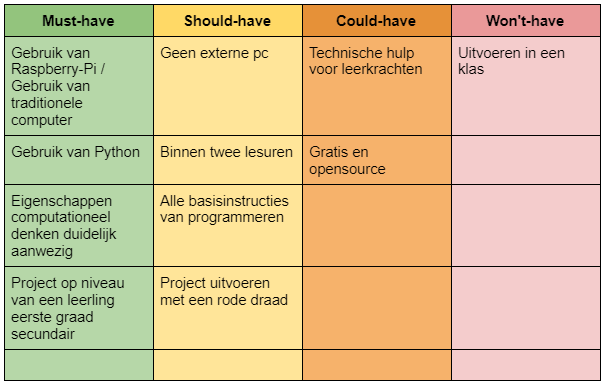
\includegraphics[width=\linewidth]{requirements}
   \caption{MoSCoW voorstelling van de requirements}
   \label{fig:moscow}
\end{figure}

\section{Long list}

We weten wat we kunnen verwachten van ons project Nu kunnen we verschillende opties proberen en evalueren of er genoeg requirements afgetikt zijn. Aangezien we al de hardware en software hebben bepaald, kunnen we makkelijk zoeken naar mogelijke projecten. Hiervoor bekijken we volgende opties:

Dankzij de website “upgrad.com”\footnote{\url{https://www.upgrad.com/blog/python-projects-ideas-topics-beginners/}} kunnen we al een paar projecten bekijken, zoals het maken van een Tic-tac-toe spel (xox). Dit kan gemaakt worden met behulp van Python en kan zeker gemaakt worden op een Raspberry Pi, maar het programmeerniveau van zo’n applicatie ligt iets te hoog voor beginnende programmeurs. 

Een andere optie is het maken van binair zoekalgoritme. Dit is een klassiek voorbeeld van een basis applicatie. Het tikt dus de box af voor het implementeren van de eigenschappen van computationeel denken en is zeker mogelijk om te maken in Python. Het is wel een minder creatieve opgave en het niveau kan soms al te hoog zijn voor leerlingen van de eerste graad.

Een contactlijst is ook een andere optie. Hierin kan iemand contactgegevens opslaan van zijn beste vriend of vriendin. Dit kan gemaakt worden in Python, maar bestaat niet echt uit de basisinstructies van programmeren en kan zelf complexere methodes opvragen. Het lijkt dus geen aantrekkelijke optie.

Dankzij een YouTube video van freeCodeCamp.org\footnote{\url{https://www.youtube.com/watch?v=8ext9G7xspg&ab_channel=freeCodeCamp.org}} kunnen we nog een paar projecten evalueren, zoals het maken van een photo processor. Hierbij kan je een foto aanpassen door bijvoorbeeld de foto waziger te maken of door de belichting te verhogen. Allemaal dankzij wat lijntjes code. Opnieuw, dit is een project dat men kan maken in Python, maar de onderdelen van computationeel denken zijn vager aanwezig. Er is een kennis van fotobewerking nodig om het probleem makkelijk te onderverdelen in kleinere problemen. Het niveau ligt dus waarschijnlijk iets te hoog.

We kunnen misschien een raadspel maken. Hierin kan de gebruiker dus proberen een getal te raden die de computer heeft gekozen of zelfs een programma maken waarmee het zelf een getal kan raden. De eigenschappen van computationeel denken zitten hier duidelijk in verwerkt. Aangezien het een spel is, heeft het dus zeker een creatieve input. Het lijkt dus een goede optie.

Verder kunnen we misschien een mad libs spel maken. Hierin vraagt de computer om bepaalde woorden zoals bijvoeglijke naamwoorden of werkwoorden die de gebruiker moet ingeven, waarna het een verhaal maakt met de ingegeven woorden. Dit is zeker een creatief project en heeft duidelijk de eigenschappen van computationeel denken in verwerkt, maar het is een wat te makkelijke opgave. Het bevat ook weinig tot bijna geen basisinstructies, zoals een voorwaarde of een lus. Minder aantrekkelijk dus.

Nog een bekend spel dat we zouden kunnen uitwerken in Python, is hangman. Hierin proberen mensen een bepaald woord te raden binnen een bepaald aantal beurten. Op zich lijkt dit een ideaal voorbeeld van een klassieke programmeeroefening. Je kan snel de eigenschappen van computationeel denken herkennen en het bevat de basisinstructies van programmeren. Een goede kandidaat dus.
Tenslotte kunnen we proberen om het klassieke blad steen schaar spel na te maken in Python. Ook hier zijn de eigenschappen van computationeel denken duidelijk aanwezig. Ook heeft het een creatieve input aan het project. Nog een geschikte kandidaat.

Nu we een lijst van potentiële opgaven hebben gemaakt, kunnen we bekijken welke projecten meer geschikt zijn voor zelf uit te voeren. Men kan in vorige oplijsting dus een drietal kandidaten uitvissen: Het getal raad spel, hangman en “blad steen schaar”. Om de meest geschikte kandidaat te bepalen, moeten we volgende projecten verder in detail bespreken.

\section{Short list}

We hebben drie projecten die we kunnen evalueren tegenover elkaar. Er zal een project uitgekozen worden om verder uit te werken in een proof of concept.

\subsection{Hangman}

Hangman is een simpel spel waarin de speler proberen een woord te raden van een medespeler. Zo moeten de speler letters raden die misschien deel vormen van het woord. Bij elk juist antwoord worden alle plaatsen waarin de letter in het woord verwerkt zit, getoond. Bij elk fout antwoord wordt er een deel van de hangman getekend. Het spel eindigt wanneer alle letters geraden zijn of wanneer de hangman volledig getekend is.

We kunnen alle aspecten van hangman bekijken om te kunnen evalueren of het een geslaagd project kan zijn. Het bevat bijvoorbeeld duidelijk de eigenschappen van computationeel denken. 

Men kan dankzij decompositie het hele spel opsplitsen in verschillende tussen problemen: de gebruiker raadt, de computer evalueert de gegeven letter, de computer “tekent” de hangman, de computer controleert als het woord geraden is, de computer toont een letter en het spel eindigt. 

Dankzij abstractie kunnen we deze problemen versimpelen. Bij de eerste stap geeft de gebruiker een letter in. Hierna controleert de applicatie of de letter aanwezig is in het woord. Wanneer de letter aanwezig is toont de applicatie het lege woord met de ingevulde letters. Hierna controleert de applicatie als alle letters geraden zijn.  Als dit zo blijkt te zijn,  stopt het spel en is de gebruiker gewonnen. Anders spelen we verder. Wanneer de letter niet te vinden is, verhogen we de 'hangman' teller. Als de teller een boven een vastgelegde waarde zit, zoals bijvoorbeeld zeven, stopt het spel en wint de computer. 

Dankzij patroonherkenning zien we dat deze fases constant herhaald worden tot het spel stopt. Ook zien we duidelijk vier verschillende fases die herhaald worden: de raad-fase, de controle-fase, de uitkomst fase en de 'einde spel'-fase. Ook bij de controle-fase gebruik gemaakt van de input van de gebruiker, dus is er sprake van een voorwaarde. De raad-fase wordt herhaald voor een onbekende duur. Dit is een voorbeeld van een while-lus. Ook kunnen we ervan uitgaan dat de controle-fase een if-instructie zal bevatten, aangezien we waardes gaan vergelijken. De 'einde spel'-fase moet controleren als het spel gedaan is en daarmee het spel stoppen. Hier lijkt een if-instructie dus ook van toepassing.

Als we nu al deze fases aan elkaar hangen op een logische manier, hebben we dankzij algoritmisch denken het hangman spel gemaakt.

Juist omdat het een bekend spel is, is er weinig vakjargon die moet aangeleerd worden bij het uitwerken van dit project. Ook maakt het gebruik van meerdere basisinstructies. 

Een probleem bij dit project kan de complexiteit zijn. Er zijn veel stappen die moeten worden doorlopen om het spel te kunnen uitspelen. Dit kan ervoor zorgen dat er sneller problemen kunnen oplopen tijdens de les. De handleiding voor de leerkracht zou al in lengte groeien. Ook zou het kunnen dat dit project langer dan twee lesuren zou duren, waardoor de vlotheid van het project een deuk neemt. 

Toch is het een goede optie om uit te werken, al dan niet in een langere periode dan twee lesuren. Het is een creatief spel waarmee de leerlingen zeker plezier mee kunnen ervaren.

\subsection{Blad Steen Schaar}

Ook 'Blad Steen Schaar' is een leuk spel om te maken op de computer. Als we de eigenschappen van computationeel denken erop laten los gaan, kunnen we bekijken als het genoeg potentieel heeft om verder uitgebouwd te worden.

Via decompositie kunnen we ook dit probleem opdelen in verschillende kleinere problemen: de speler speelt, de computer speelt, de computer evalueert de beide keuzes en een punt wordt gegeven aan de winnaar. Eventueel kan je de 'beste uit drie'-regel toepassen en het spel laten stoppen binnen drie beurten. Hierbij komt de stap erbij dat de computer controleert als het spel gedaan is.

Via abstractie kunnen we deze deelproblemen verder uitwerken. Bij de eerste stap vraagt de computer om een input van de gebruiker: blad, steen of schaar. Hierna geeft de gebruiker één van deze keuzes in. Hierna kiest de computer een willekeurige zet. In de volgende stap bekijkt de computer met een legende wie gewonnen heeft en geeft de winnaar een punt. Wanneer men binnen drie beurten speelt, kan de computer nog evalueren als het spel afgelopen is. Zo zou het spel stoppen wanneer een van beide partijen een 2-0 heeft of wanneer iemand een hogere score heeft na drie zetten.

Via patroonherkenning zien we in dat er bepaalde fases worden doorlopen: de keuze-fase, de punten-fase en de controle-fase. Deze worden steed opnieuw herhaald. Ook stopt het spel na drie beurten en wordt de input van de gebruiker verwerkt, wat wijst op een if-voorwaarde. Tenslotte worden deze fases in chronologische volgorde uitgevoerd, ook al kan men beslissen om eerst de computer te laten kiezen en dan pas de gebruiker.
Dankzij algoritmen kunnen deze fases aan elkaar worden gekoppelt voor een volledig resultaat. 

In tegenstelling tot het hangman spel is dit een korter project om uit te werken. Hierdoor is het makkelijker om uit te voeren in de klas en om het binnen de periode van twee lesuren te houden. Dankzij de simpliciteit van 'Blad steen schaar' is er ook minder uitleg nodig voor leerlingen en leerkrachten.

Deze simpliciteit heeft echter zijn nadelen. 'Blad steen schaar' is nogal simpel en misschien niet zo interessant voor leerlingen om zich daar twee lesuren mee bezig te houden. Maar zelfs met de negatieve aspecten lijkt blad steen schaar een goede keuze om te gebruiken tijdens de lessen computationeel denken.

\section{Proof of concept: Raadspel}

De proof of concept voor dit onderzoek bestaat uit het opstellen van een lesvoorbereiding voor het raadspel met gebruik van Python en een Raspberry Pi. Hierna zal de uitvoering van de lesvoorbereiding gemaakt worden op zowel een traditionele computer als een Raspberry Pi. Hieruit kunnen we een SWOT-analyse opstellen en evalueren of de Raspberry Pi een meerwaarde geeft in de lessen programmeren in de eerste graad van het secundair onderwijs.

\subsection{Lesvoorbereiding}
Als deel van de proof of concept, wordt er een lesvoorbereiding gemaakt voor het maken van een Raadspel. Dit zal volledig gemaakt worden in Python en zal in de SWOT-analyse uitgevoerd worden op zowel een Raspberry Pi als een klassieke computer. Hieruit zullen we kunnen bekijken wat de gebruikerservaring van een Pi is.

Om een project om te vormen naar een lesactiviteit, is een lesvoorbereiding van cruciaal belang. Alleen zo geef je een project wat structuur en maak je het makkelijker voor de leerkracht om te evalueren als je opdracht alle einddoelen aftikt.

Deze \ref{ch:lesvoorbereiding} is te vinden na de methodologie.

\subsection{SWOT-analyse Raspberry Pi}

Zoals eerder vermeld heeft, bestaat de proof of concept uit een vergelijking met traditionele computers zoals een desktop of laptop. Hiervoor zullen dezelfde stappen uitgevoerd worden op zowel de Pi als de klassieke computer. Beide scenario’s worden los van elkaar uitgevoerd, maar moeten identiek en repliceerbaar zijn.

We belichten eerst de sterke eigenschappen van het programmeren met een Pi. 
Het startscherm van de Raspberry Pi is enorm herkenbaar in vergelijking met andere besturingssystemen. Er was geen nood aan het opzoeken van een handleiding om te kunnen starten. Dankzij de duidelijke gebruikersinterface kan je makkelijk de ingebouwde browser vinden, een tekstbestand opstellen, files aanmaken, uw mappen organiseren en veel meer. Het aanpassen van de schermresolutie was ook intuïtief. Alle interactie schermen zijn minimalistisch en to-the-point. Wanneer men toch hulp nodig heeft, kan je makkelijk een handleiding aanroepen via het startmenu, te herkennen aan het Raspberry logo in de taakbalk. Dit maakt het besturingssysteem aanzienlijk gebruiksvriendelijker dan klassieke UI’s, zoals Microsoft Windows, die soms met hun vele features de gebruikers kan afschrikken.

Voor dagdagelijkse praktijken zoals een word document opstellen, kan je snel de “Office”-knop indrukken in het startmenu om de Pi variant van Microsoft Office te gebruiken: LibreOffice. Deze applicaties zijn gratis en komen geïnstalleerd bij het besturingssysteem. Dit komt steeds minder vaak voor in de wereld van de klassieke computers. Bij Windows moet men zelf betalen voor deze features. Dit maakt de Raspberry Pi een interessante concurrent op vlak van office-tools.

De Raspberry Pi OS maakt het makkelijk om snel een project te starten via de startmenu. Door door te klikken op de programmeren optie kan je makkelijk Thonny vinden en opstarten. Klassieke besturingssystemen hebben vaak geen voorgeïnstalleerde IDE. De instapklare eigenschap van de Pi is dus zeker een pluspunt. 

Zoals eerder vermeld, wordt er gebruik gemaakt van Thonny: een gebruiksvriendelijke en simpele IDE die standaard geïnstalleerd is op de Raspberry Pi OS. Deze IDE maakt gebruik van een duidelijk en minimalistische gebruikersinterface om zo snel mogelijk van slag te gaan. Je krijgt meteen twee schermen te zien: het script en de shell. Via het script kan je makkelijk je project beginnen programmeren en via de shell kan je het script runnen. Er zitten ook handige features in zoals een debug mode en een code correctie hulp die u code controleert en feedback geeft over wat er beter kan. 

De gebruikerservaring bij het programmeren zelf is praktisch en gestroomlijnd. Dankzij de snelknoppen naar de IDE en de simpele gebruikersinterface kan je snel een project opstarten en uitvoeren.


De Pi toont zijn lelijke kantjes wanneer je het wilt gebruiken voor meer dan simpele programmeer sessies. Dankzij zijn gelimiteerde hardware en features kan de gebruikservaring snel dalen wanneer je een Pi gebruikt voor meer alledaagse activiteiten zoals youtube video’s bekijken. Door de gelimiteerde hardware kan de Pi moeilijk image en video processing aan, waardoor youtube video’s vaak haperen en streaming praktisch onmogelijk lijkt. 

Ter verdediging van de Raspberry Pi: dit kan liggen aan de externe hardware waarmee de Pi verbonden is. Met een ander, kleiner computerscherm was er minder hapering vastgesteld, maar nog steeds hapering in het algemeen. Het is dus sterk afhankelijk van de verbonden hardware. Belangrijk om te weten wanneer je beseft dat een leerkracht vaak wisselt tussen een normaal scherm en een beamer.

Zoals vermeld heeft de Pi al verschillende, voorgeïnstalleerde programma's voor dagdagelijkse activiteiten zoals LibreOffice, maar ook deze hebben problemen. De gebruikersinterface lijkt enorm gedateerd en onaantrekkelijk. Door het gebruiksvriendelijk te maken worden vaak vele handige features geschrapt. Het mist bijvoorbeeld veel layout opties die standaard zijn bij Word, zoals het vrij aanpassen en toevoegen van stijlen. 
Dit probleem is niet enkel te zien bij LibreOffice. Heel wat onderdelen van het besturingssysteem voelen gedateerd en gelimiteerd aan. 

Dankzij de gelimiteerde hardware is de Pi ook gevoelig aan lag: het proces waarbij programma's trager aanvoelen of vaak blokkeren. Tijdens het gebruik van de browser kan men vaak langer wachten op zoekresultaten dan bij een klassieke browser. Ook dit heeft een negatief effect op de gebruikerservaring van de Pi.

De grootste slag in het gezicht bij de Pi is iets wat je niet direct zou aan denken met een klassieke pc, maar toch o zo belangrijk is: de stroomtoevoer. Aangezien de Pi zijn stroomtoevoer krijgt van een USB-C of Micro-USB kabel, is het gevoelig aan wisselingen in voltage. Bij het opladen van een gsm is dit minder merkbaar, maar bij het volledig draaien van een computer is dit duidelijk merkbaar. Wanneer de Pi detecteert dat er te weinig stroomtoevoer binnen vloeit in het apparaat, geeft het een melding die om de vijf minuten terugkeert. Hierbij vraagt het om uw Raspberry Pi te verbinden met een sterkere stroombron. Dit kan echter aan veel onderdelen liggen, van de adapter waarmee je het in het stopcontact steekt tot het stopcontact in kwestie. Het is dus onvoorspelbaar als uw Pi genoeg stroom zal krijgen om te blijven doorwerken.

Wanneer de Pi te veel activiteiten tegelijk moet draaien op een lage energiebron, kan het spontaan uitvallen en opnieuw opstarten. Dit heeft een drastisch effect op je workflow en de gebruikerservaring. Wanneer de Pi opnieuw opstart, kan het niet garanderen dat al uw werk van vooraf opgeslagen blijft. Hierdoor kan de gebruiker uren van werk kwijtraken. 
Maar dit is nog niet het ergste aspect van een stroomuitval. Zoals vermeld in de literatuurstudie, heeft de Pi geen functie waarbij het lopende processen eerst afsluit voordat het stroom verliest. Hierdoor kan niet enkel uw files beschadigt raken, maar zelfs uw hele besturingssysteem, waardoor je al uw werk compleet kan kwijtraken. Dit is een gigantische dreun in het gezicht van de Raspberry Pi.  

Los van deze tekortkoming heeft de Pi toch nog kansen om verder uit te groeien naar een goede substitutie voor een klassieke computer in de klassfeer. De Raspberry Pi foundation en zijn actieve community zijn nog altijd bezig met het verbeteren van de Pi ervaring. Er komen nog steeds nieuwe modellen op de markt, met de Pi 400 speciaal ontworpen om de normale desktop of laptop te vervangen. Met de jaren kunnen we betere prestatie verwachten en zou het weleens een rol kunnen spelen in het onderwijs.
Zoals vermeld zijn er actieve communities die ofwel proberen het bestaande besturingssysteem te optimaliseren oftewel totaal nieuwe besturingssystemen introduceren zoals Linux. 

De Pi vecht momenteel wat tegen de bierkaai als het probeert om traditionele computers te vervangen. Eenmaal het verbeterd in prestaties of grafische capaciteiten, zijn klassieke pc's al uitgerust met nog nooit geziene snelheden en prestaties. Ook genieten single board computers nog niet van de bekendheid die moderne smart apparaten wel hebben. Het blijft een wat nich concept voor velen. Zoals eerder vermeld bij het kiezen van een single board computer zijn leerkrachten nog niet overtuigd om het te implementeren in de klas.





%%=============================================================================
%% Lesvoorbereiding
%%=============================================================================

\chapter{\IfLanguageName{dutch}{Lesvoorbereiding}{Lesson preparation}}
\label{ch:lesvoorbereiding}

Dit onderdeel van het onderzoek bestaat uit een lesvoorbereiding van het besproken raadspel. Dit bestaat uit een inleiding, een probleemstelling, een uitwerking en conclusie. Deze lesvoorbereiding werd verstuurd naar verschillende leerkrachten in de eerste graad secundair onderwijs. Deze leerkrachten hebben al ervaring met het implementeren van computationeel denken in hun lessen. Er werd hun gevraagd of de lesvoorbereiding zou werken in de praktijk (in een echte les). 

\section{Document}

\subsection{Inleiding en voorwoord}
Ik wil u persoonlijk bedanken voor uw interesse in mijn bachelorproef. Uw feedback op dit project zal een grote bijdrage leveren aan mijn onderzoek. Op het einde van dit document vraag ik u om uw feedback. Als u en uw feedback wenst anoniem te blijven in mijn paper, is dit zeker mogelijk, op aanvraag.

De bedoeling was om dit project uit te voeren in een klas. Spijtig genoeg, door de huidige covid-situatie en een tekort aan hardware, leek dit plan onrealistisch. Om dit project toch les-klaar te maken, heb ik besloten om een lesvoorbereiding te schrijven die de leerdoelen aangrijpt en het project uitlegt, stap per stap.

Dit document is onderdeel van mijn bachelorproef en bestaat uit een lesvoorbereiding voor een python project. Dit project wordt uitgevoerd op een Raspberry Pi, een minicomputer speciaal gemaakt om te leren programmeren. Dit project tackelt de eindtermen over Digitale Competentie en Media wijsheid, en specifieker de einddoelen van computationeel denken. Dit is geen erkende lesvoorbereiding en zou dus elementen kunnen missen.

Aan het einde van dit voorstel vraag ik u om uw feedback. Dit kan gaan van diepgaande feedback over de inhoud tot meer oppervlakkige kritiek. Op het einde vraag ik u of uw dit project realistisch vindt in een klassfeer en als u dit zelf zou willen uitvoeren met een Raspberry Pi. Deze feedback ontvang ik graag via mail: warre.vandeveire@gmail.com.

Nogmaals bedankt voor uw interesse en tijd,
Warre Van de Veire

\subsection{Overzicht van project}
Dit project bestaat uit het maken van een Python applicatie die een getal kan raden van een gebruiker. 
Zo moet de gebruiker bij de start van het spel een getal kiezen tussen 1 en 100. Hierna zal de computer een willekeurig getal presenteren. De gebruiker moet hierop feedback geven. Zo kan de gebruiker kiezen tussen drie opties: hoger, lager of correct. Wanneer de gebruiker hoger of lager ingeeft, zal de computer de feedback toepassen en een nieuwe gok wagen. Wanneer de gebruiker “correct” ingeeft, stopt het spel en presenteert de computer het correct geraden getal.

Dit project maakt gebruik van de Python programmeertaal en een Raspberry Pi. In de bijlage van deze lesvoorbereiding zit een beschrijving van de Raspberry Pi en de programmeertaal in kwestie. 
Dit document bestaat uit een introductie op het project, de probleemstelling, de uitwerking en een conclusie. Deze stappen zijn noodzakelijk voor het slagen van mijn onderzoek en de verwerking ervan in een klassfeer. 

\subsection{Uitdagingen}
\begin{itemize}
    \item Gebruik van de text-based programmeertaal: Python
    \item Gebruik van basis-instructies:
    \subitem Een lus
    \subitem Een voorwaarde
    \subitem een sequentie
    \subitem Gebruikersinput
    \item Gebruik van de Raspberry Pi
\end{itemize}

\subsection{Doelstellingen}
\begin{itemize}
    \item Verwerven van de competenties rond computationeel denken
\end{itemize}

\subsection{Voorkennis}
\begin{itemize}
    \item Basisinstructies van Python
    \subitem 'If'-voorwaarde
    \subitem 'While'-voorwaarde
    \subitem Variabelen
    \subitem Input
\end{itemize}

\subsection{Vereisten/taken}
\begin{enumerate}
    \item Alle onderdelen van computationeel denken moeten duidelijk aanwezig zijn in het project:
    \subitem Decompositie
    \subitem Abstractie
    \subitem Patroonherkenning
    \subitem Algoritmes
    \item Er mag zo weinig mogelijk gebruik gemaakt van vaktermen. Zo moet dit project uitvoerbaar blijven voor leerkrachten met een minimum aan programmeerkennis.
    \item De stappen voor het uitwerken van deze opdracht moeten duidelijk uitgelegd worden, waardoor er weinig nood is externe hulp.
    \item Het project moet uitvoerbaar zijn op een Raspberry Pi en moet de programmeertaal Python gebruiken.
    \item Het uitvoeren van het project mag niet langer dan twee lesuren duren: 2x50min.
    \item Het project moet een creatieve ingeving hebben en moet interessant blijven voor de leerlingen van de eerste graad.
\end{enumerate}

\subsection{Uitwerking}
\subsubsection{Introductie van het project}
\emph{Om het project te introduceren, lijkt het goed om luchtig te starten. We moeten dit ook kunnen terugkoppelen naar een probleem in de realiteit. Zo kunnen we gebruik maken van de eigenschappen van computationeel denken om aan te tonen dat dit vaak in de realiteit, onbewust, wordt gebruikt.}

Start de les met het spelen van het raadspel, zonder gebruik te maken van de computer. De leerkracht kan oftewel zelf een getal proberen te raden van een student of omgekeerd. De bedoeling is dat de leerling een idee krijgt hoe het spel werkt. 

Na een paar keer te spelen, zal de leerkracht opnieuw het spel uitvoeren, maar nu met behulp van het uitgewerkte project. Zo moet een leerling een getal verzinnen tussen 1 en 100 en moet de computer het raden. Nu de leerling het spel snapt en het uitgewerkte project in actie heeft gezien, kunnen we verdergaan naar de probleemstelling.

\subsubsection{Probleemstelling}
\emph{In dit onderdeel zullen we bespreken wat we precies willen bereiken en hoe we dit kunnen aanpakken. Hierin maken we gebruik van decompositie om de opdracht op te delen in kleinere, sub problemen. Hierna kunnen we, dankzij abstractie, deze kleinere problemen versimpelen. Dankzij patroonherkenning kunnen we deze problemen omvormen naar gelijkaardige oplossingen. Na we alle stappen hebben aangehaald, kunnen we deze stappen op een logische manier sorteren en gieten in een algoritme. Hiermee is het probleem opgelost en hebben we ons project gemaakt.}

We kunnen het gehele spel onderverdelen in verschillende, kleinere problemen. We starten bij het identificeren van de rollen. Probeer hiermee af te vragen wie er speelt. Zo kan de speler een groep leerlingen zijn of een enkele. We proberen dit echter simpel te houden, dus kiezen we voor één gebruiker.

\underline{Vragen:}
\begin{itemize}
    \item Wie speelt het spel?
    \item Welke partijen zijn hierbij betrokken?
\end{itemize}
\underline{Oplossing:}
\begin{itemize}
    \item Rol 1: De speler $\rightarrow$ leerling
    \item Rol 2: De rader $\rightarrow$ computer
\end{itemize}

Nu we de rollen hebben geïdentificeerd, kunnen we bekijken wat elke rol precies uitvoert. Som alle acties op die de rollen uitvoeren bij het maken van dit project. Plaats deze acties onder de rol.

\underline{Vragen:}
\begin{itemize}
    \item Welke acties voeren deze rollen uit doorheen het spel?
    \item Communiceren deze rollen met elkaar?
\end{itemize}
\underline{Oplossing:}
Zie figuur \ref{fig:lesvoor_prob1}

\begin{figure}
    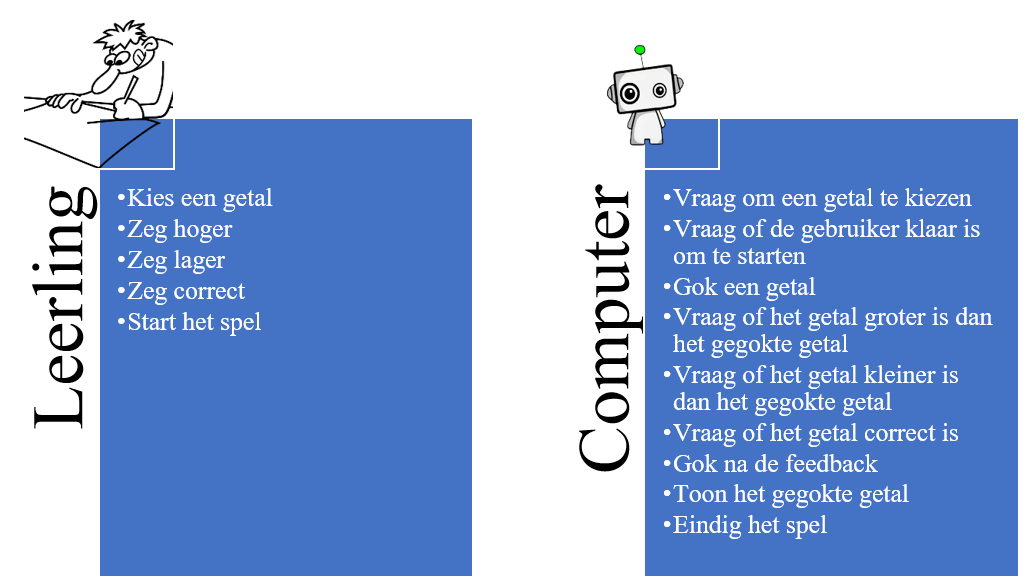
\includegraphics[width=\linewidth]{probleemstelling1}
    \caption{Alle acties per rol}
    \label{fig:lesvoor_prob1}
\end{figure}

Nu we de rollen duidelijk kennen en de acties die worden uitgevoerd, kunnen we deze problemen versimpelen door bepaalde acties onder een noemer te plaatsen. Aangezien de computer de meeste taken heeft, zal er vooral bij deze rol versimpelt moeten worden. Dit maakt het project makkelijker te begrijpen en haalt de complexiteit ervan weg. Dankzij abstractie kunnen we bijvoorbeeld bepaalde taken groeperen onder één actie.

\underline{Vragen:}
\begin{itemize}
    \item Welke acties kunnen we groeperen?
    \item Welke acties kunnen we tegelijkertijd uitvoeren doorheen het spel?
    \item Welke acties zijn noodzakelijk voor het uitvoeren van het spel en welke kunnen we weglaten?
\end{itemize}
\underline{Oplossing:}
Zie figuur \ref{fig:lesvoor_prob2}

\begin{figure}
    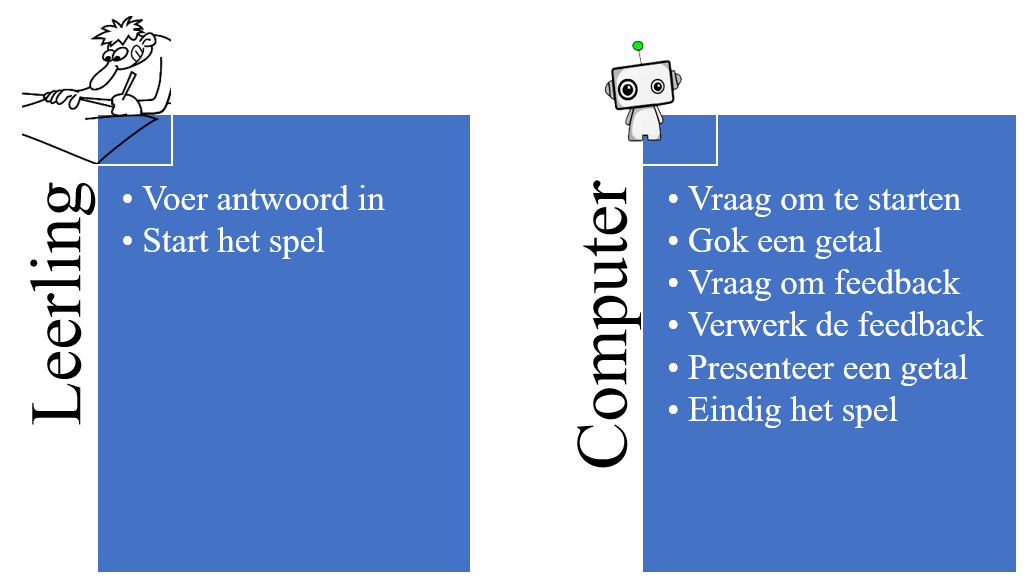
\includegraphics[width=\linewidth]{probleemstelling2}
    \caption{Alle versimpelde acties per rol}
    \label{fig:lesvoor_prob2}
\end{figure}

Nu we duidelijk de rollen en de acties hebben opgesomd, kunnen we alles in een logische volgorde gieten. Maak een schema op met de logische volgorde. Zet hierbij ook de juiste instructies om zo de link met Python makkelijker te maken. Met patroonherkenning kunnen we bijvoorbeeld inzien dat we werken met een lus van onbepaalde duur.

\underline{Vragen:}
\begin{itemize}
    \item Welke acties volgen elkaar op?
    \item Welke acties worden herhaald?
    \item Moet een rol wachten op de actie van een andere rol?
    \item Zijn er acties die tegelijk lopen?
    \item Welke acties hebben invloed op elkaar?
\end{itemize}
\underline{Oplossing:}
Zie figuur \ref{fig:lesvoor_prob3}

\begin{figure}
    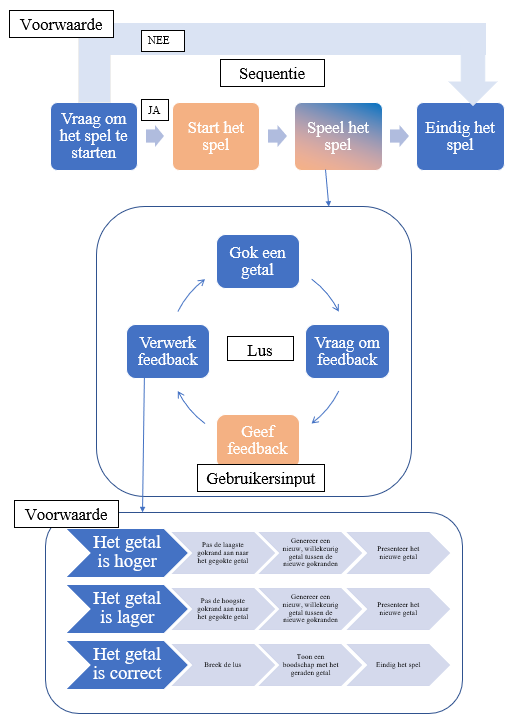
\includegraphics[width=\linewidth]{probleemstelling3}
    \caption{Uitgewerkt overzicht met alle acties, op logische volgorde}
    \label{fig:lesvoor_prob3}
\end{figure}

Dankzij de eigenschappen van computationeel denken hebben we nu een simpel raadspel opgedeeld en uitgewerkt. Nu we weten wat er precies uitgevoerd moet worden, kunnen we starten met het uitwerken van dit spel in Python.

\subsubsection{Uitwerking}
\emph{We zullen het proces, uitgewerkt in de probleemstelling, nu maken in Python. Hiervoor maken we gebruik van een Raspberry Pi als computer en Thonny als IDE. Thonny is een beginnersvriendelijke ontwikkelomgeving speciaal ontworpen voor de Raspberry Pi. We gaan elke stap in de probleemstelling omvormen naar Python code om een werkende applicatie te bekomen. In figuur \ref{fig:lesvoor_rasp1} en figuur \ref{fig:lesvoor_rasp2} kunt u zien hoe u Thonny gebruikt op een Raspberry Pi:}

\begin{figure}
    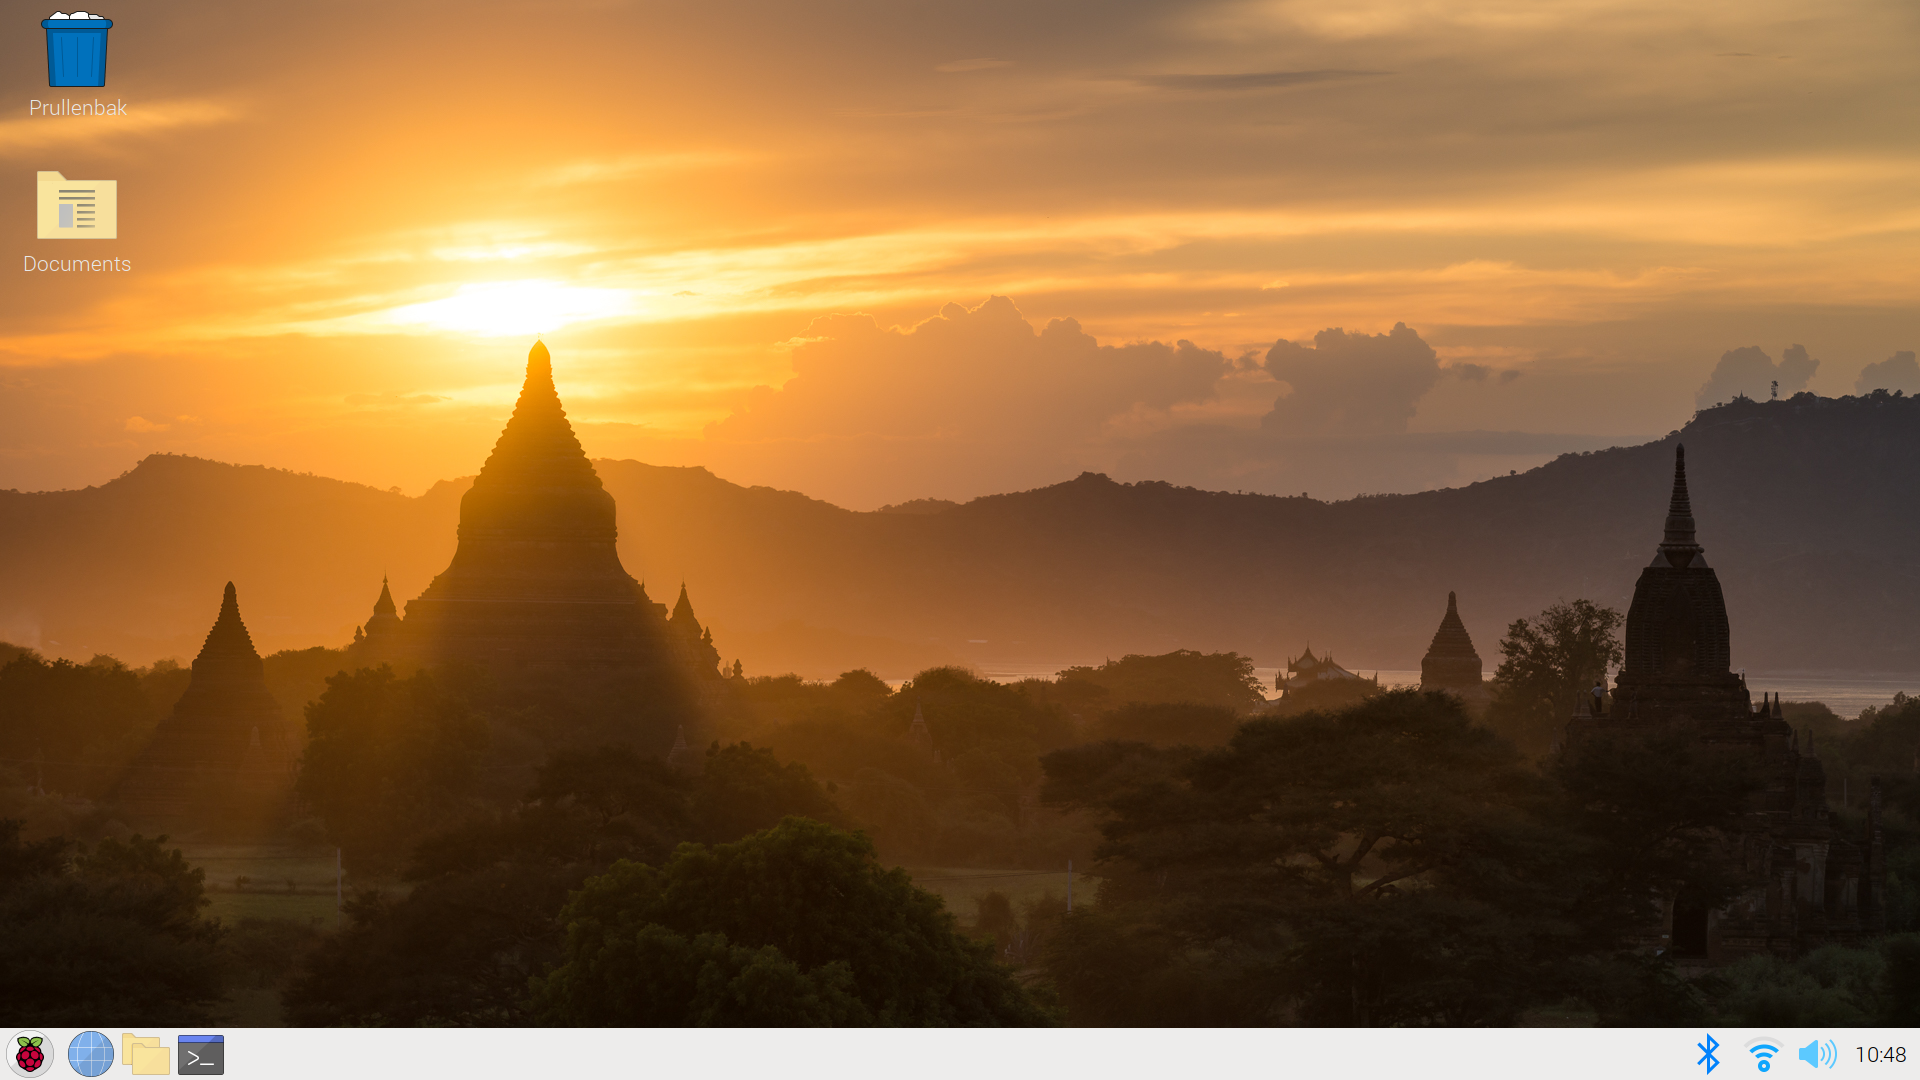
\includegraphics[width=\linewidth]{lesvoorbereidingPi1}
    \caption{Opstartscherm van de Raspberry Pi OS}
    \label{fig:lesvoor_rasp1}
\end{figure}

\begin{figure}
    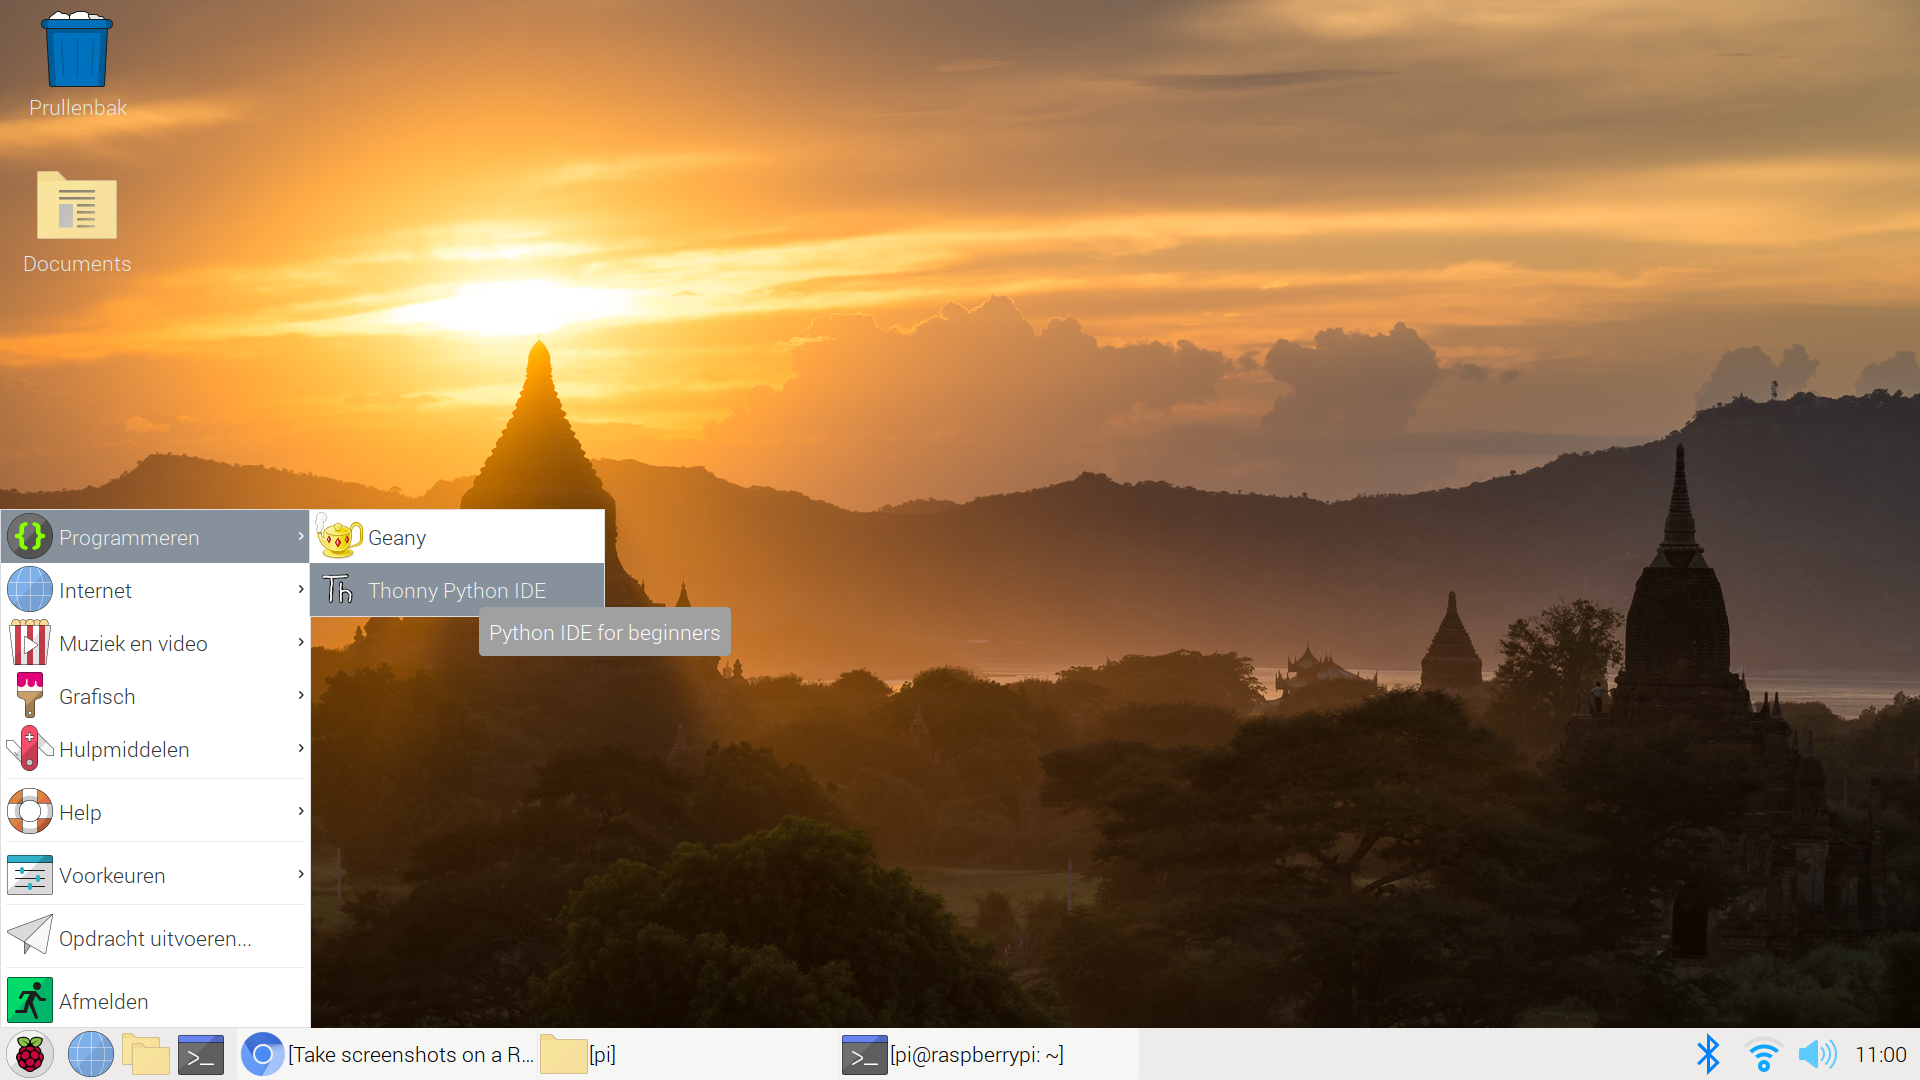
\includegraphics[width=\linewidth]{lesvoorbereidingPi2}
    \caption{Openen van Thonny via het startmenu}
    \label{fig:lesvoor_rasp2}
\end{figure}

We starten eerst met de opbouw van de Python applicatie. Dit begint bij het maken van een methode en dan hierop verder te bouwen. We starten vanuit de sequentie en gaan zo dieper in de applicatie. 

\emph{Bij het starten van Thonny krijgt u dit scherm te zien (zie figuur \ref{fig:uitwerking1} ):
    U ziet direct twee schermen: het script scherm en de shell. In het script scherm zullen de leerlingen hun code schrijven. Dankzij de shell zullen de leerlingen het spel kunnen spelen.}

\begin{figure}
    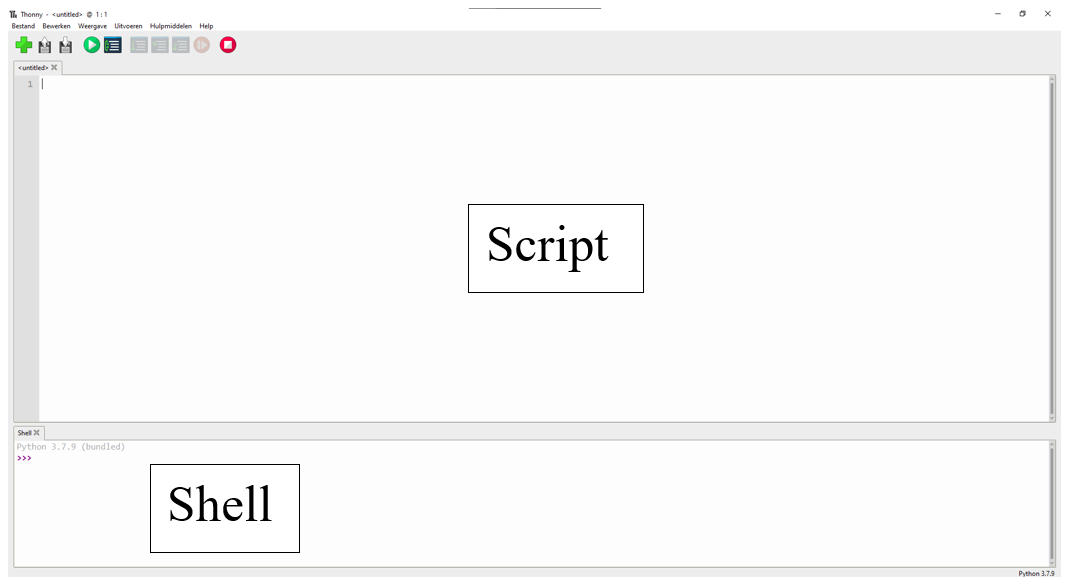
\includegraphics[width=\linewidth]{uitwerking1}
    \caption{Thonny startscherm}
    \label{fig:uitwerking1}
\end{figure}

Het volledige uitgewerkte project zal er uiteindelijk zo uit zien:
\begin{lstlisting}[language=Python, caption=Volledige uitwerking van het raadspel in Python]
import random

def raadspel():
    print(f"Welkom bij het raad spel! Kies een getal tussen 1 en 100: ")
    startSpel = input("Als je klaar bent om te beginnen, druk 'j'. Als je wilt stoppen, druk 'n'.").capitalize()

    if startSpel == "J":
        print(f"{startSpel}")
        lageRand = 1
        hogeRand = 100
        feedback = ""
        teller = 0
        while(feedback!="G"):
            print(f"Ik denk dat jouw getal ligt tussen {lageRand} en {hogeRand}. Ik heb momenteel {teller} keer geraden.")
            gok = random.randint(lageRand, hogeRand)
            feedback = input(f"Is jouw getal hoger (H) of lager (L) dan {gok}? Of heb ik het getal geraden? (G)?: ").capitalize()
            if feedback == "L":
                hogeRand = gok-1
            elif feedback == "H":
                lageRand = gok+1
            teller=teller+1
        print(f"Yay, we hebben jouw getal ({gok} geraden) in {teller} beurten!")

    print("Vaarwel :)")

raadspel()
\end{lstlisting}

\underline{De sequentie + voorwaarde}

We zullen eerst de hoofdsequentie omvormen. Deze start de applicatie spel, vraagt om een input en stopt het spel.

We hebben dus nood aan een inputwaarde. In Python wordt dit gedefinieerd door een variabele gelijk te stellen aan een input methode. We geven in de haakjes van de input een boodschap mee die de gebruiker uitlegt wat te doen (zie figuur \ref{fig:uitwerking2}):

\begin{figure}
    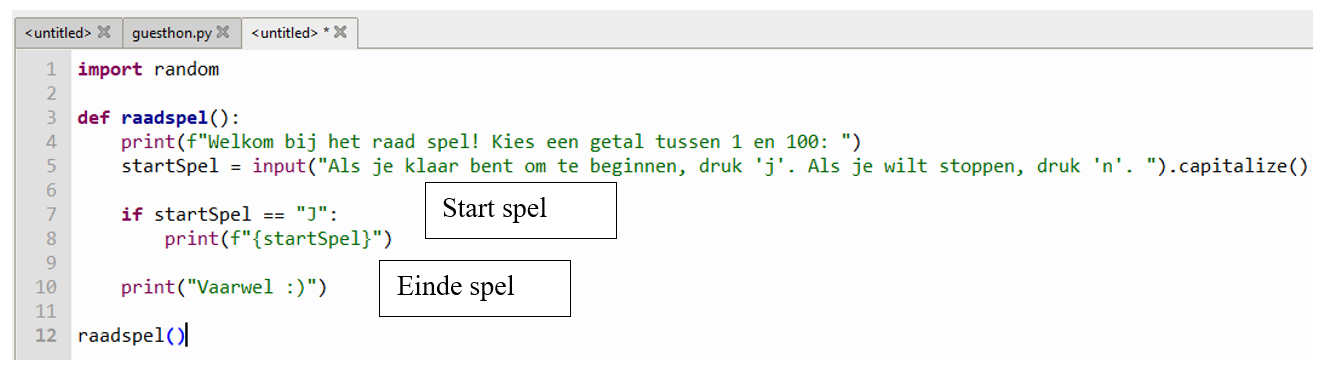
\includegraphics[width=\linewidth]{uitwerking2}
    \caption{Eerste stap uitgewerkt: sequentie + voorwaarde}
    \label{fig:uitwerking2}
\end{figure}

\textbf{UITBREIDING}: Dankzij de 'capitalize()'-methode, zal de input omgezet worden naar hoofdletters. Dit zorgt ervoor dat de gebruiker zowel een kleine letter 'j' als grote letter 'J' kan ingeven, aangezien het allemaal omgezet wordt naar grote letters.

Dankzij de 'if'-instructie kunnen we een voorwaarde toevoegen. Bij deze voorwaarde bekijkt hij als de input gelijk is aan 'J'. 
Dankzij de print('…') methode kunnen we een melding weegeven.

\textbf{UITBREIDING}: Je kan ook de waarde van 'startSpel' weergeven. Hierbij zetten we een f voor de aanhalingstekens en zetten we de waarde omringt door gekrulde haakjes. 

Wanneer de gebruiker nu 'J' ingeeft, ziet hij de input. Wanneer hij een andere letter ingeeft, stopt het spel.

\underline{De lus}

Nu we het spel kunnen starten, zullen we beginnen met het implementeren van de lus. De computer gaat constant vragen om feedback tot het getal geraden is. Hij zal dus bepaalde stukken code herhalen voor een onbepaalde duur: we weten op voorhand niet hoeveel keer de computer zal nodig hebben om het getal te raden.  

In de voorwaarde zullen we nu een lus toevoegen. Eerst hebben we nood aan variabelen die onze zoekranden bijhoudt. Er is nood aan een hoge en lage rand. 
Er is ook nood aan een feedback variabele. Hierin zal de gebruiker dus zijn antwoord kunnen meegeven.
Tenslotte kunnen we een teller toevoegen die controleert hoeveel pogingen de computer nodig had om het getal te raden. Zie figuur \ref{fig:uitwerking3}:

\begin{figure}
    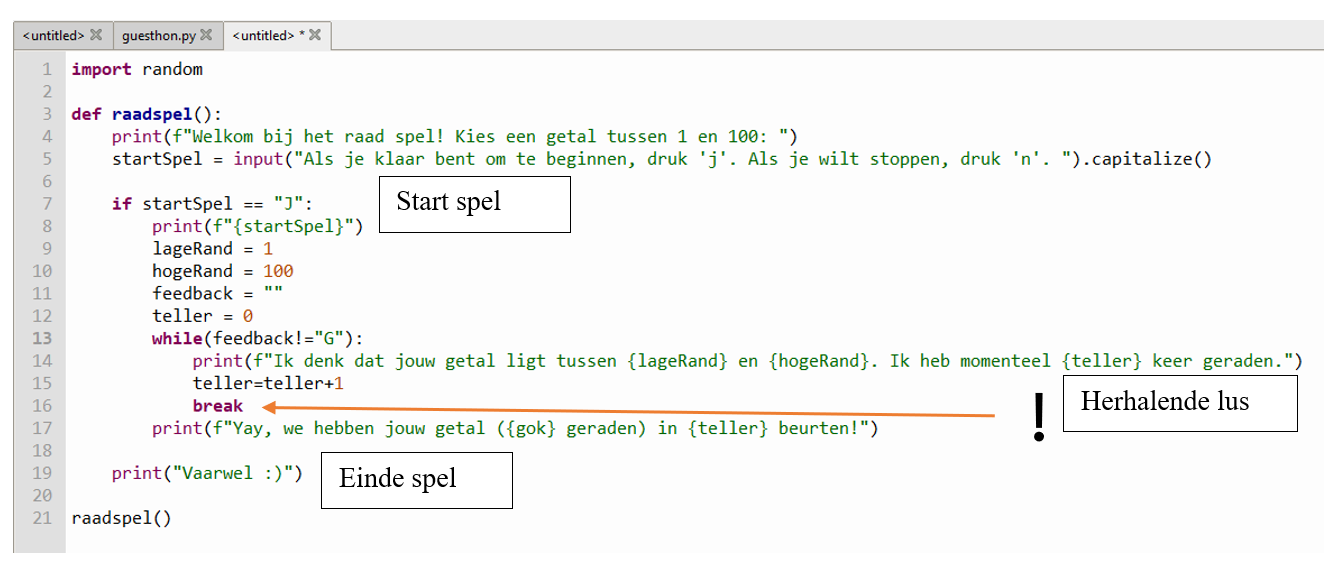
\includegraphics[width=\linewidth]{uitwerking3}
    \caption{Tweede stap uitgewerkt: de lus}
    \label{fig:uitwerking3}
\end{figure}

Zoals eerder vermeld gebruiken we een hoge en lage zoekrand. Deze zijn bij het begin van het zoeken 1 en 100, aangezien ons zoekveld ligt tussen deze waarden.
Het feedback veld blijft nu even leeg. We vragen nog niet aan de gebruiker als het getal hoger of lager ligt.
De teller heeft ook een standaardwaarde. Deze zal verhoogd worden bij elke lus.

Aangezien we niet weten hoe vaak de computer gaat proberen te raden, zullen we een 'while'-instructie gebruiken. Zolang de voorwaarde in de haakjes klopt, worden de instructies vanbinnen herhaald. 
Wanneer deze voorwaarde niet meer klopt, stopt de lus.
In ons geval zal de lus stoppen wanneer de variabele 'feedback' gelijk is aan 'G'. 
Met de syntax binnen de haakjes wordt dus verteld: 
zolang feedback NIET GELIJK AAN (!=) 'G' is, zal de lus opnieuw doorlopen worden.

\textbf{BELANGRIJK}: aangezien we momenteel de feedback niet aanpassen, zal deze lus in de oneindigheid blijven doorlopen. Het is dus belangrijk om een 'break' te plaatsen op het einde van de lus. Dit breekt sowieso de lus, los van de verklaring tussen de haakjes.

\underline{De gebruikersinput: gokken en het ingeven van feedback}
We hebben een lus die wacht op de feedback van de gebruiker. Nu moeten we dus feedback kunnen geven op een gok. We zullen dus de computer een variabele “gok” laten bijhouden die een willekeurige waarde tussen de zoekranden genereert (zie figuur \ref{fig:uitwerking4}):

\begin{figure}
    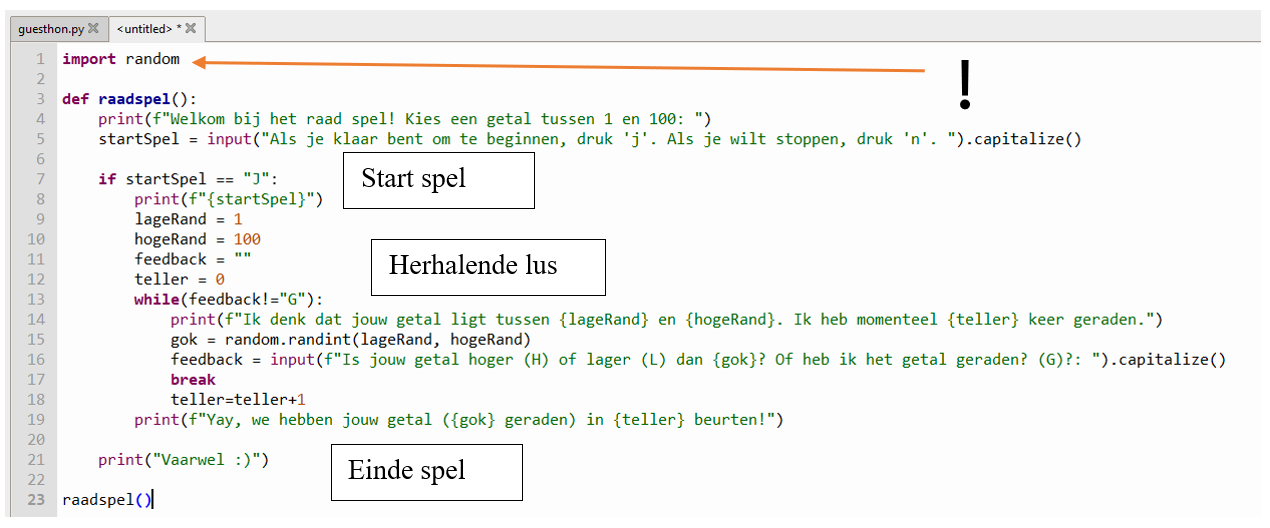
\includegraphics[width=\linewidth]{uitwerking4}
    \caption{Derde stap uitgewerkt: de gebruikersinput}
    \label{fig:uitwerking4}
\end{figure}

Zoals je kunt zien, de computer maakt een willekeurig getal aan dankzij de hoge en lage zoekrand. Dit doen we dankzij het geïmporteerde object: random. De methode 'randint' genereert dit willekeurig getal. Dankzij de argumenten tussen deze haakjes weet de methode randint() tussen welke waarden het getal moet gekozen worden.

Pas nadat de computer een gok heeft gemaakt, kan het vragen om feedback aan de gebruiker. We passen dus de waarde aan van feedback, dankzij een tweede input. Ook deze input zullen we in hoofdletters omvormen.

\underline{Geavanceerdere voorwaarden: feedback verwerken en zoekranden aanpassen}

We krijgen feedback binnen van de gebruiker. Deze kan oftewel hoger (H), lager (L) of geraden (G) antwoorden. Aangezien de lus zal beëindigd worden bij het invoeren van G, moeten we hiervoor geen voorwaarde schrijven. We moeten wel de zoekranden aanpassen wanneer de gebruiker hoger of lager ingeeft. Zie figuur \ref{fig:uitwerking5}:

\begin{figure}
    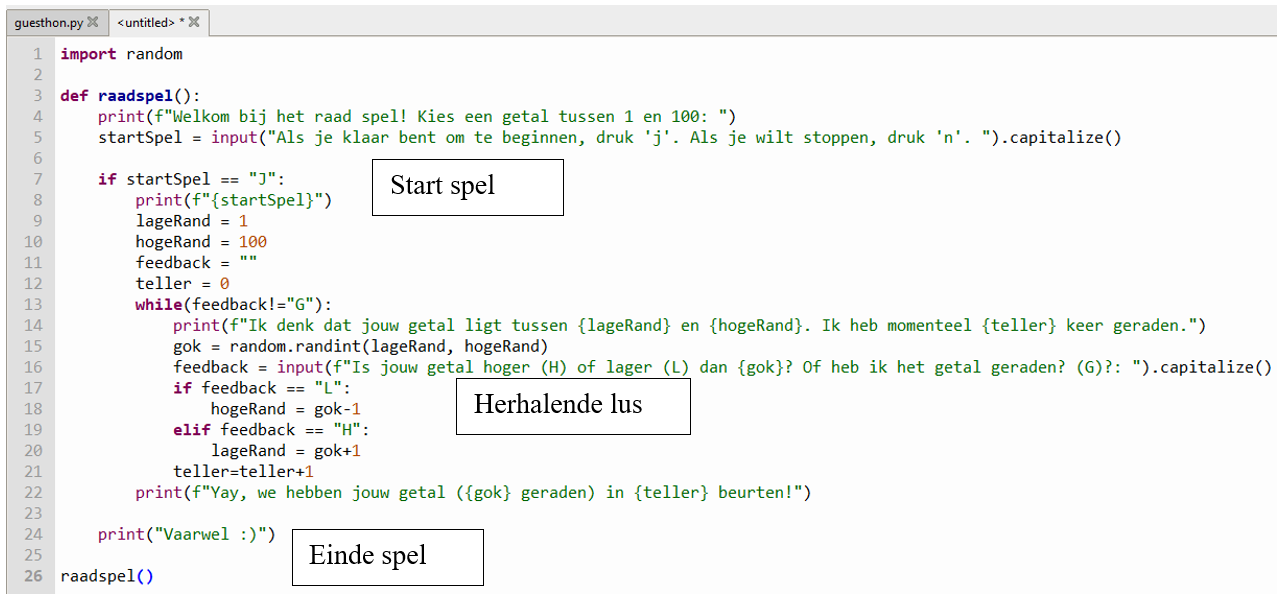
\includegraphics[width=\linewidth]{uitwerking5}
    \caption{Vierde stap uitgewerkt: Geavanceerde voorwaarden}
    \label{fig:uitwerking5}
\end{figure}

In dit geval maken we gebruik van een tweedelige voorwaarde. We bekijken eerst als de ingegeven feedback \emph{lager} was. Wanneer dit het geval is, passen we onze hoge zoekrand aan naar de gegokte waarde. Het te zoeken getal is nl. kleiner dan de huidige bovengrens (opgeslagen in de variabel \emph{hogeRand})
We trekken er nog één vanaf, aangezien we de gegokte waarde niet willen toevoegen in het zoekgebied.

Als de computer ziet dat de gebruiker geen 'L' heeft ingegeven, zal het bekijken als de feedback een 'H' is. Dit vind je terug in het tweede deel van de voorwaarde (elif). Als de echte waarde groter is dan de gegokte waarde, zal het de \emph{lage zoekrand} aanpassen. Ook dit keer willen we de gokwaarde niet opnemen in het zoekgebied.

Nu is ons raadspel zo goed als af. We moeten enkel nog een boodschap meegeven die ons vertelt dat het getal geraden is en in hoeveel beurten. Deze boodschap moet slechts 1 maal afgedrukt worden, aan het einde van het spel
We voegen daarom een print() methode uit BUITEN de lus.

En zo is het project afgewerkt. Als een leerling op de speel-knop drukt (groene pijl links-bovenaan, zie figuur \ref{fig:uitwerking1}), start het spel in de shell. Volg de instructies en laat de computer uw getal raden.

\emp{UITBREIDING}: Het spel werkt, maar is nog niet fout-vriendelijk. Als je per ongelijk een verkeerd antwoord ingeeft, is de kans groot dat het gekozen getal niet meer in het zoekgebied ligt. Ook zou het kunnen dat de hoge zoekrand lager komt te liggen dan de lage zoekrand. Dit zou het spel breken. Met het volgende stukje code toe te voegen, zou je dit probleem kunnen vermijden:

\begin{lstlisting}[language=Python, caption=Volledige uitwerking van het raadspel in Python]
if lageRand == hogeRand:
    gok = hogeRand
else:
    gok = random.randint(lageRand, hogeRand)
\end{lstlisting}

\subsubsection{Conclusie}
We hebben succesvol een raadspel kunnen maken in Python. Dankzij de eigenschappen van computationeel denken hebben we dit probleem makkelijk kunnen ontleden en omvormen naar leesbare code.

\subsection{Bedanking}
Ik bedank nogmaals uw interesse in mijn bachelorproef. Als u feedback zou hebben op dit document, stuur mij graag een bericht voor 28/05/2021 om 12u via warre.vandeveire@gmail.com 

Bedankt en nog een prettige dag.

\subsection{Bijlage}
\emph{\underline{Raspberry Pi:}} 
De Raspberry Pi is een single board computer: een volledige functionele computer op een enkele printplaat.
Opgericht in 2008 als liefdadigheidsinstelling in het Verenigd Koninkrijk, staat de Raspberry Pi Foundation in voor het verspreiden van computationele en digitale kennis over de hele wereld. Zo organiseert Raspberry verschillende workshops en events om het potentieel van de Raspberry Pi te demonstreren.
Ook moedigt Raspberry verschillende scholen over de hele wereld aan om gebruik te maken van hun technologie in de klas. Zo wil het niet alleen programmeren populair maken, maar wil het ook technologie introduceren in andere wetenschappelijk vakken zoals fysica of chemie.

\emph{\underline{Python:}}
Python is een klassieke text-based programmeertaal. De gebruiker schrijft zelf de instructies uit die de computer moet uitvoeren. Dit, in tegenstelling tot Scratch, is de meest gebruikte vorm van programmeren en is de norm in de professionele wereld. Python is een open-source codetaal: iedereen mag er gratis gebruik van maken, zonder te betalen.
Dit is niet zo abnormaal in de wereld van codetalen. Wat Python uniek maak, is zijn lage complexiteit. In tegenstelling tot bekende programmeertalen zoals Java, is gemakkelijk te lezen en is de instap veel lager.


\section{Feedback}
Zoals eerder vermeld, werd deze lesvoorbereiding verstuurd naar verschillende leerkrachten in de hoop om hun feedback te ontvangen.
De belangrijkste vragen waren als volgt:
\begin{itemize}
    \item Vind u deze les realistisch in een les in de eerste graad?
    \item Zou u het zien zitten om dit project uit te werken met behulp van een Raspberry Pi en Python?
\end{itemize}
Na het ontvangen van een aantal kritische kijken kunnen we evalueren als ons onderzoek zou slagen in de praktijk. 

De algemene consensus was dat het project interessant lijkt en zeker leuk om uit te voeren in de les. Ook was de lesvoorbereiding goed opgesteld en werden de eigenschappen van computationeel denken duidelijk uitgewerkt. Tenslotte leek het werken met een Raspberry Pi een interessante uitdaging. 

Het probleem viel bij de meeste leerkrachten bij de keuze van programmeertaal, namelijk Python.
Volgens Sean Callens ligt het probleem vooral bij de syntax-kennis. Om Python correct te kunnen gebruiken, heb je nood aan een voorkennis over de specifieke syntax. Dit zou in de praktijk een te groot obstakel kunnen vormen voor leerlingen van de eerste graad. Callens stelt dus voor om dit eerder te organiseren in een tweede graad. Scratch zou, volgens Callens, een veel intuïtievere programmeertaal zijn. Hierbij kan er nadruk gelegd worden op het probleemoplossend gedeelte van programmeren, zonder de leerlingen te belasten met syntax-kennis en foutbestendigheid. 

% Voeg hier je eigen hoofdstukken toe die de ``corpus'' van je bachelorproef
% vormen. De structuur en titels hangen af van je eigen onderzoek. Je kan bv.
% elke fase in je onderzoek in een apart hoofdstuk bespreken.

%\input{...}
%\input{...}
%...

%%=============================================================================
%% Conclusie
%%=============================================================================

\chapter{Conclusie}
\label{ch:conclusie}

% TODO: Trek een duidelijke conclusie, in de vorm van een antwoord op de
% onderzoeksvra(a)g(en). Wat was jouw bijdrage aan het onderzoeksdomein en
% hoe biedt dit meerwaarde aan het vakgebied/doelgroep? 
% Reflecteer kritisch over het resultaat. In Engelse teksten wordt deze sectie
% ``Discussion'' genoemd. Had je deze uitkomst verwacht? Zijn er zaken die nog
% niet duidelijk zijn?
% Heeft het onderzoek geleid tot nieuwe vragen die uitnodigen tot verder 
%onderzoek?

\lipsum[76-80]



%%=============================================================================
%% Bijlagen
%%=============================================================================
\appendix
\renewcommand{\chaptername}{Appendix}

%%---------- Onderzoeksvoorstel -----------------------------------------------

\chapter{Onderzoeksvoorstel}

Het onderwerp van deze bachelorproef is gebaseerd op een onderzoeksvoorstel dat vooraf werd beoordeeld door de promotor. Dat voorstel is opgenomen in deze bijlage. 

% Verwijzing naar het bestand met de inhoud van het onderzoeksvoorstel
%---------- Inleiding ---------------------------------------------------------

\section{Introductie} % The \section*{} command stops section numbering
\label{sec:introductie}

Hier introduceer je werk. Je hoeft hier nog niet te technisch te gaan.

Je beschrijft zeker:

\begin{itemize}
  \item de probleemstelling en context
  \item de motivatie en relevantie voor het onderzoek
  \item de doelstelling en onderzoeksvraag/-vragen
\end{itemize}

%---------- Stand van zaken ---------------------------------------------------

\section{State-of-the-art}
\label{sec:state-of-the-art}

Hier beschrijf je de \emph{state-of-the-art} rondom je gekozen onderzoeksdomein. Dit kan bijvoorbeeld een literatuurstudie zijn. Je mag de titel van deze sectie ook aanpassen (literatuurstudie, stand van zaken, enz.). Zijn er al gelijkaardige onderzoeken gevoerd? Wat concluderen ze? Wat is het verschil met jouw onderzoek? Wat is de relevantie met jouw onderzoek?

Verwijs bij elke introductie van een term of bewering over het domein naar de vakliteratuur, bijvoorbeeld~\autocite{Doll1954}! Denk zeker goed na welke werken je refereert en waarom.

% Voor literatuurverwijzingen zijn er twee belangrijke commando's:
% \autocite{KEY} => (Auteur, jaartal) Gebruik dit als de naam van de auteur
%   geen onderdeel is van de zin.
% \textcite{KEY} => Auteur (jaartal)  Gebruik dit als de auteursnaam wel een
%   functie heeft in de zin (bv. ``Uit onderzoek door Doll & Hill (1954) bleek
%   ...'')

Je mag gerust gebruik maken van subsecties in dit onderdeel.

%---------- Methodologie ------------------------------------------------------
\section{Methodologie}
\label{sec:methodologie}

Hier beschrijf je hoe je van plan bent het onderzoek te voeren. Welke onderzoekstechniek ga je toepassen om elk van je onderzoeksvragen te beantwoorden? Gebruik je hiervoor experimenten, vragenlijsten, simulaties? Je beschrijft ook al welke tools je denkt hiervoor te gebruiken of te ontwikkelen.

%---------- Verwachte resultaten ----------------------------------------------
\section{Verwachte resultaten}
\label{sec:verwachte_resultaten}

Hier beschrijf je welke resultaten je verwacht. Als je metingen en simulaties uitvoert, kan je hier al mock-ups maken van de grafieken samen met de verwachte conclusies. Benoem zeker al je assen en de stukken van de grafiek die je gaat gebruiken. Dit zorgt ervoor dat je concreet weet hoe je je data gaat moeten structureren.

%---------- Verwachte conclusies ----------------------------------------------
\section{Verwachte conclusies}
\label{sec:verwachte_conclusies}

Hier beschrijf je wat je verwacht uit je onderzoek, met de motivatie waarom. Het is \textbf{niet} erg indien uit je onderzoek andere resultaten en conclusies vloeien dan dat je hier beschrijft: het is dan juist interessant om te onderzoeken waarom jouw hypothesen niet overeenkomen met de resultaten.



%%---------- Andere bijlagen --------------------------------------------------
% TODO: Voeg hier eventuele andere bijlagen toe
%\input{...}

%%---------- Referentielijst --------------------------------------------------


\printbibliography[heading=bibintoc]

\end{document}
